% ============================================================
\section{Experiments and Case Studies}
\label{sec:eval}
% ============================================================

We evaluate the LDM through three case studies that cover distinct structured search domains. \S\ref{sec:autoresearch} presents an autonomous-research loop over neural-network training programs \citep{karpathy2026autoresearch}; \S\ref{sec:cs-antibody-results} demonstrates the competitive performance of LDM in antibody CDRH3 sequence design \citep{khan2022antbo}; and \S\ref{sec:cs-molecule-results} attests to the effectiveness of LDM in multi-objective small-molecule drug discovery against the KRAS G12D target \citep{kumarOverviewKRASG12D2026}. \S\ref{sec:finetune-experiments} then distils the LDM test-time search policy into a reusable proposer across all three domains, and \S\ref{sec:ablation-main} isolates which components of LDM actually drive the gains. Together, these studies evaluate the framework across program search, biological sequence design, and molecular design, employing common baselines, ablations, metrics, and falsifiable hypotheses where applicable.

\subsection{Autonomous research loop}
\label{sec:autoresearch}
% ============================================================

\begin{figure}[ht]
    \centering
    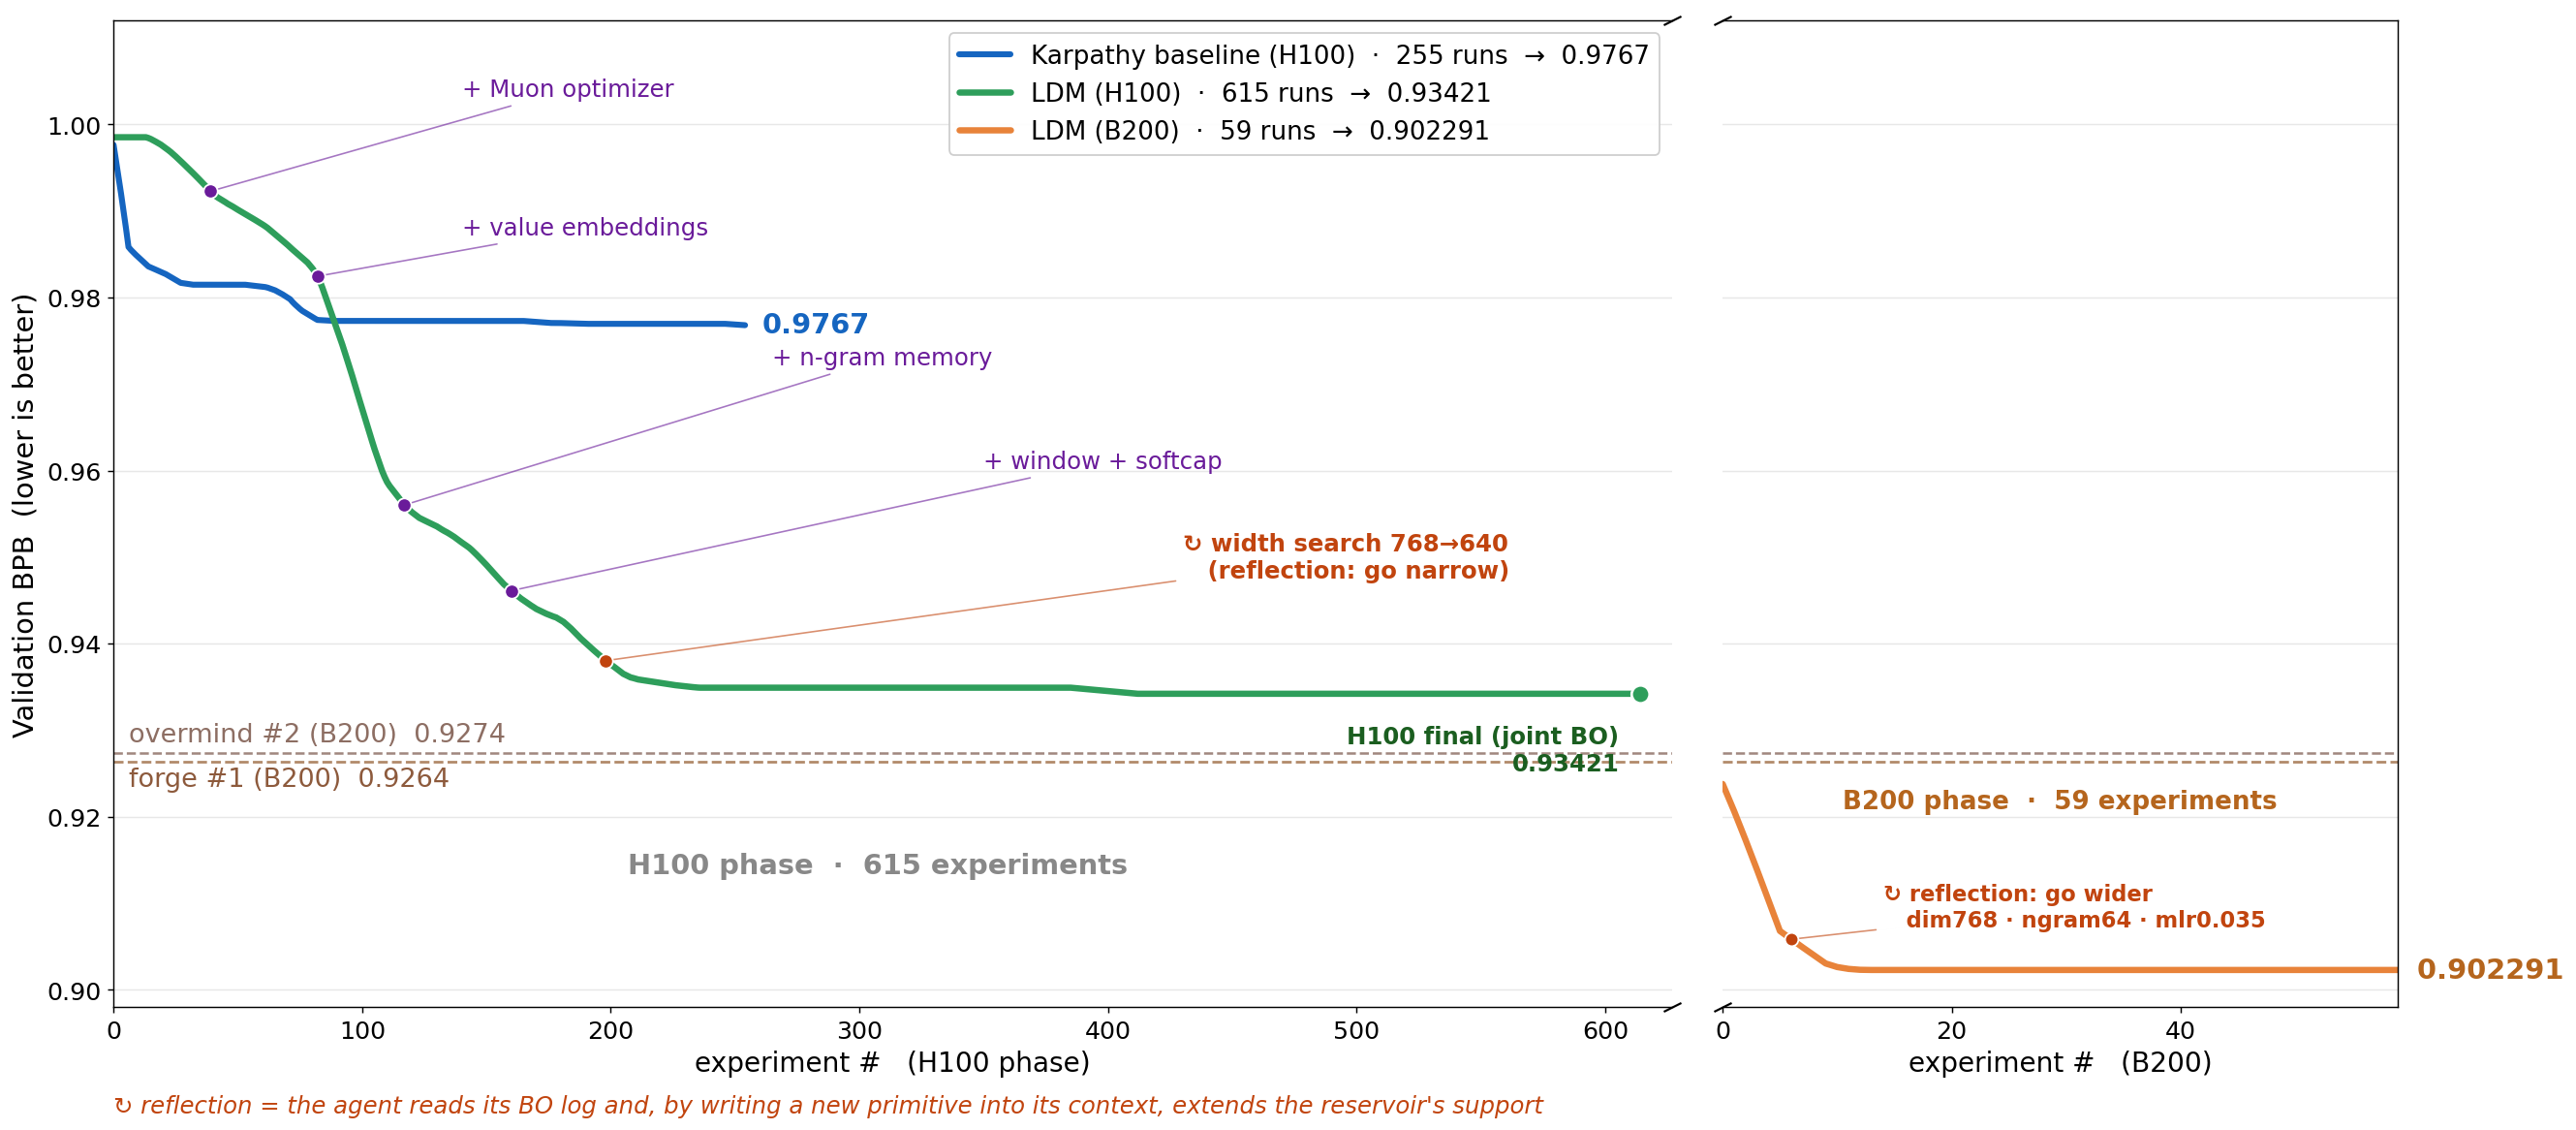
\includegraphics[width=0.95\linewidth]{figure/ldm_h100_b200.png}
    \caption{\textbf{The discover loop on \texttt{autoresearch}.} Validation \texttt{val\_bpb} (lower is better) versus search progress. The H100 panel compares the no-discover Karpathy baseline with the LDM; the B200 panel reports a matched-hardware leaderboard run of the LDM. B200 width scaled for legibility.}
    \label{fig:autoresearch}
\end{figure}

\begin{table}[ht]
\centering
\footnotesize
\begin{tabular}{@{}llr@{}}
\toprule
Change & Why it helps under a fixed time budget & $\Delta$\texttt{val\_bpb} \\
\midrule
$n$-gram hash memory             & memorises local $n$-gram patterns at zero FLOP     & $-0.0275$ \\
QK-norm                          & steadier steps, more learning per step             & $-0.0137$ \\
Narrower model (dim 768$\to$640) & cheaper steps $\Rightarrow$ more steps in 300\,s   & $-0.0109$ \\
Windowed attention + softcap     & cheaper attention $\Rightarrow$ more tokens/sec    & $-0.0108$ \\
Squared-ReLU                     & richer per-token MLP representation                & $-0.0087$ \\
Value embeddings                 & extra per-token signal at near-zero cost           & $-0.0079$ \\
Muon optimizer                   & orthogonalised gradients, more learning per token  & $-0.0048$ \\
\bottomrule
\end{tabular}
\caption{\textbf{The \texttt{autoresearch} run as physics-grounded discovery.} Each row lists a change the LDM retained under a fixed 300\,s budget, the physical mechanism by which it helps, and the resulting change in \texttt{val\_bpb}.}
    \label{tab:autoresearch-discovery}
\end{table}

We use Karpathy's public \texttt{autoresearch} project \citep{karpathy2026autoresearch} as a testbed for acquisition-guided LLM search. In \texttt{autoresearch}, a coding agent repeatedly modifies a single file, \texttt{train.py}; each candidate program is evaluated by training a small language model for a fixed five-minute budget and measuring validation bits per byte (\texttt{val\_bpb}, lower is better). The original system provides only the LLM proposal-and-evaluation loop, to which we add the surrogate and acquisition-guided search. Under the LDM notation, a program is a design $x$ with reward
\[
R(x)=-\texttt{val\_bpb}(x),
\]
where the agent conditioned on the current context defines the proposal distribution $p_\theta(\cdot\mid\mathcal C_t)$, and the accumulated program--performance pairs form the dataset $\mathcal D_t$ used to fit the surrogate. The benchmark is well suited to LDM: the search space is executable programs (a natural semantic proposal target), every proposal receives a quantitative but non-differentiable score from a real training run, the fixed schedule makes runs directly comparable under fixed hardware, and the full trace of edits, outcomes, and failures can be logged and ablated end to end.

\subsubsection{Experiment setting}

We instantiate LDM in the indirect-parameterisation mode: rather than generating raw program text, the LLM acts as a meta-planner that exposes the tunable degrees of freedom of \texttt{train.py} (learning rate, width, depth, and related hyperparameters) as a continuous search space, over which we establish a standard Gaussian process with an RBF kernel and fixed hyperparameters (kept fixed rather than fit, for stability in the small-data regime), giving a calibrated posterior mean and uncertainty $(\mu_t,\sigma_t)$; Expected Improvement (Eq.~\eqref{eq:ei}) serves as the acquisition function.

Each round the LLM proposes a pool of candidate configurations conditioned on $\mathcal C_t$, and the surrogate selects the next configuration to evaluate by maximising EI, with a diversity term for batched rounds. When the incumbent stalls, the reflection step lets the LLM re-parameterise the search space (i.e., adding or reshaping the tunable axes) before search resumes. The primary comparison holds the coding model, environment, and five-minute-per-run budget fixed, contrasting the original Karpathy LLM-only loop against the full LDM.

\subsubsection{Results}

Under a fixed context $\mathcal C_t$, acquisition-guided search exploits high-performing configurations and explores regions of high surrogate uncertainty. Figure~\ref{fig:autoresearch} shows the resulting \emph{descend--plateau--descend} pattern (i.e., improvement, plateau, then further improvement once reflection reshapes the search space) consistent with the intended search--stagnation--reflection cycle, though the learning curve alone does not establish causality. Under the same H100 five-minute-per-run schedule, the Karpathy LLM-only baseline plateaus at $\texttt{val\_bpb}\approx0.9767$ after about $255$ runs, whereas the full LDM continues improving to $0.93421$. This is a system-level comparison and is not intended to isolate any single component. The per-factor ablations appear in Section~\ref{sec:ablation-main} and Appendix~\ref{app:ablation}. Additionally, in Appendix~\ref{app:abl-pure-llm}, we also report the performance of the pure-LLM discovery loop, which identifies that quantification acquisition values are the central source of the LDM's advantage.

Separately, and independent of the mechanism above, Figure~\ref{fig:autoresearch} also reports a leaderboard result on B200 hardware for comparison with stronger public systems on the same accelerator. On B200 the LDM reaches $\texttt{val\_bpb}=0.902291$ in $59$ runs, surpassing the strongest public methods \textsc{forge} ($0.9264$) and \textsc{overmind} ($0.9274$) for top-1 on the \texttt{autoresearch@home} leaderboard.\footnote{\url{https://www.ensue-network.ai/lab/autoresearch}} Under the fixed training budget the model is token-bound, so \texttt{val\_bpb} falls only by training on more tokens or by learning more from each token; Table~\ref{tab:autoresearch-discovery} traces how each retained change does one or the other, taking \texttt{val\_bpb} from $0.9961$ to $0.902291$ ($-0.094$ overall), each attributable to a concrete physical mechanism rather than metric overfitting.


\subsection{Antibody CDRH3 design}
\label{sec:cs-antibody-results}

We select antibody CDRH3 loop design as our second case study because it represents a canonical high-dimensional combinatorial optimisation problem with a well-defined design space. The CDRH3 loop is the primary determinant of antibody binding specificity, with sequences of length \(L \approx 11\) drawn from 20 amino acids, yielding a discrete space of size \(20^{11}\). This setting falls into the \emph{known unknown} regime: the syntax and boundaries of the design space are fully specified, but the sequence-to-affinity mapping is unknown, highly rugged, and expensive to evaluate. Traditional combinatorial Bayesian optimisation methods struggle with the intractable size of this discrete space, while pure LLM generation lacks calibrated value guidance. The task therefore provides a clean testbed for evaluating how LDM combines structured proposal generation with calibrated acquisition guidance.

We use the \textsc{Absolut!} structure-based simulator as the black-box oracle, which returns a lattice binding energy \(E_{\mathrm{bind}}\) \citep{khan2022antbo}. We maximise \(R(x) = -E_{\mathrm{bind}}(x)\) since lower binding energy corresponds to stronger affinity, and each evaluation constitutes a single expensive oracle call.

\subsubsection{Experimental settings}

Experiments run sequentially, with one antibody candidate selected per iteration. We evaluate across five PDB targets, including 1ADQ\_A, 1FBI\_X, 1H0D\_C, 1NSN\_S, and 1OB1\_C, with a total budget of 200 evaluations per target, reporting mean performance and one standard deviation over multiple random seeds.

Baselines fall into four categories: \textbf{Pure LLM} (direct autoregressive sequence generation), combinatorial BO frameworks (\textbf{TURBO}, \textbf{COMBO}) adapted for discrete sequence spaces, the domain-specialised \textbf{AntBO} optimiser, and naive random search. We position LDM as a competitive general-purpose alternative rather than claiming to outperform the domain-specialised AntBO.

We implement four LDM variants formed by two orthogonal design choices: two LLM base generation strategies, paired with two acquisition weighting rules. Here \textbf{Policy} denotes the indirect parameterisation of \S\ref{sec:algo}: the LLM parameterises a sampling policy (with internal complexity), and the policy implicitly induces the base measure $p_{\theta,\alpha}(\cdot\mid\C_t)$. The \textbf{Direct} base measure generates sequences token-by-token with a small sample pool of \(m=5\). The \textbf{Policy} base measure lets the LLM output structured search parameters to spawn a much larger candidate pool. For weighting, \textbf{Max} picks the highest-acquisition candidate (mode approximation), while \textbf{Softmax} samples proportionally to exponentiated acquisition scores to approximate the full tilted distribution. Table~\ref{tab:ldm-variants-antibody} summarises all combinations.

\begin{table}[htbp]
    \centering
    \begin{tabular}{ccc}
        \hline
        LDM Variant & Base Measure \(p_\theta(x \mid \mathcal{C}_t)\) & Reduction Rule \\
        \hline
        Direct\_Max & Direct token-level sequence generation & Max \\
        Direct\_Softmax & Direct token-level sequence generation & Softmax \\
        Policy\_Max & Structured search policy from LLM output & Max \\
        Policy\_Softmax & Structured search policy from LLM output & Softmax \\
        \hline
    \end{tabular}
    \caption{Implemented LDM algorithm variants for computational antibody design.}
    \label{tab:ldm-variants-antibody}
\end{table}

\subsubsection{Results}

\begin{figure}[h!]
\centering
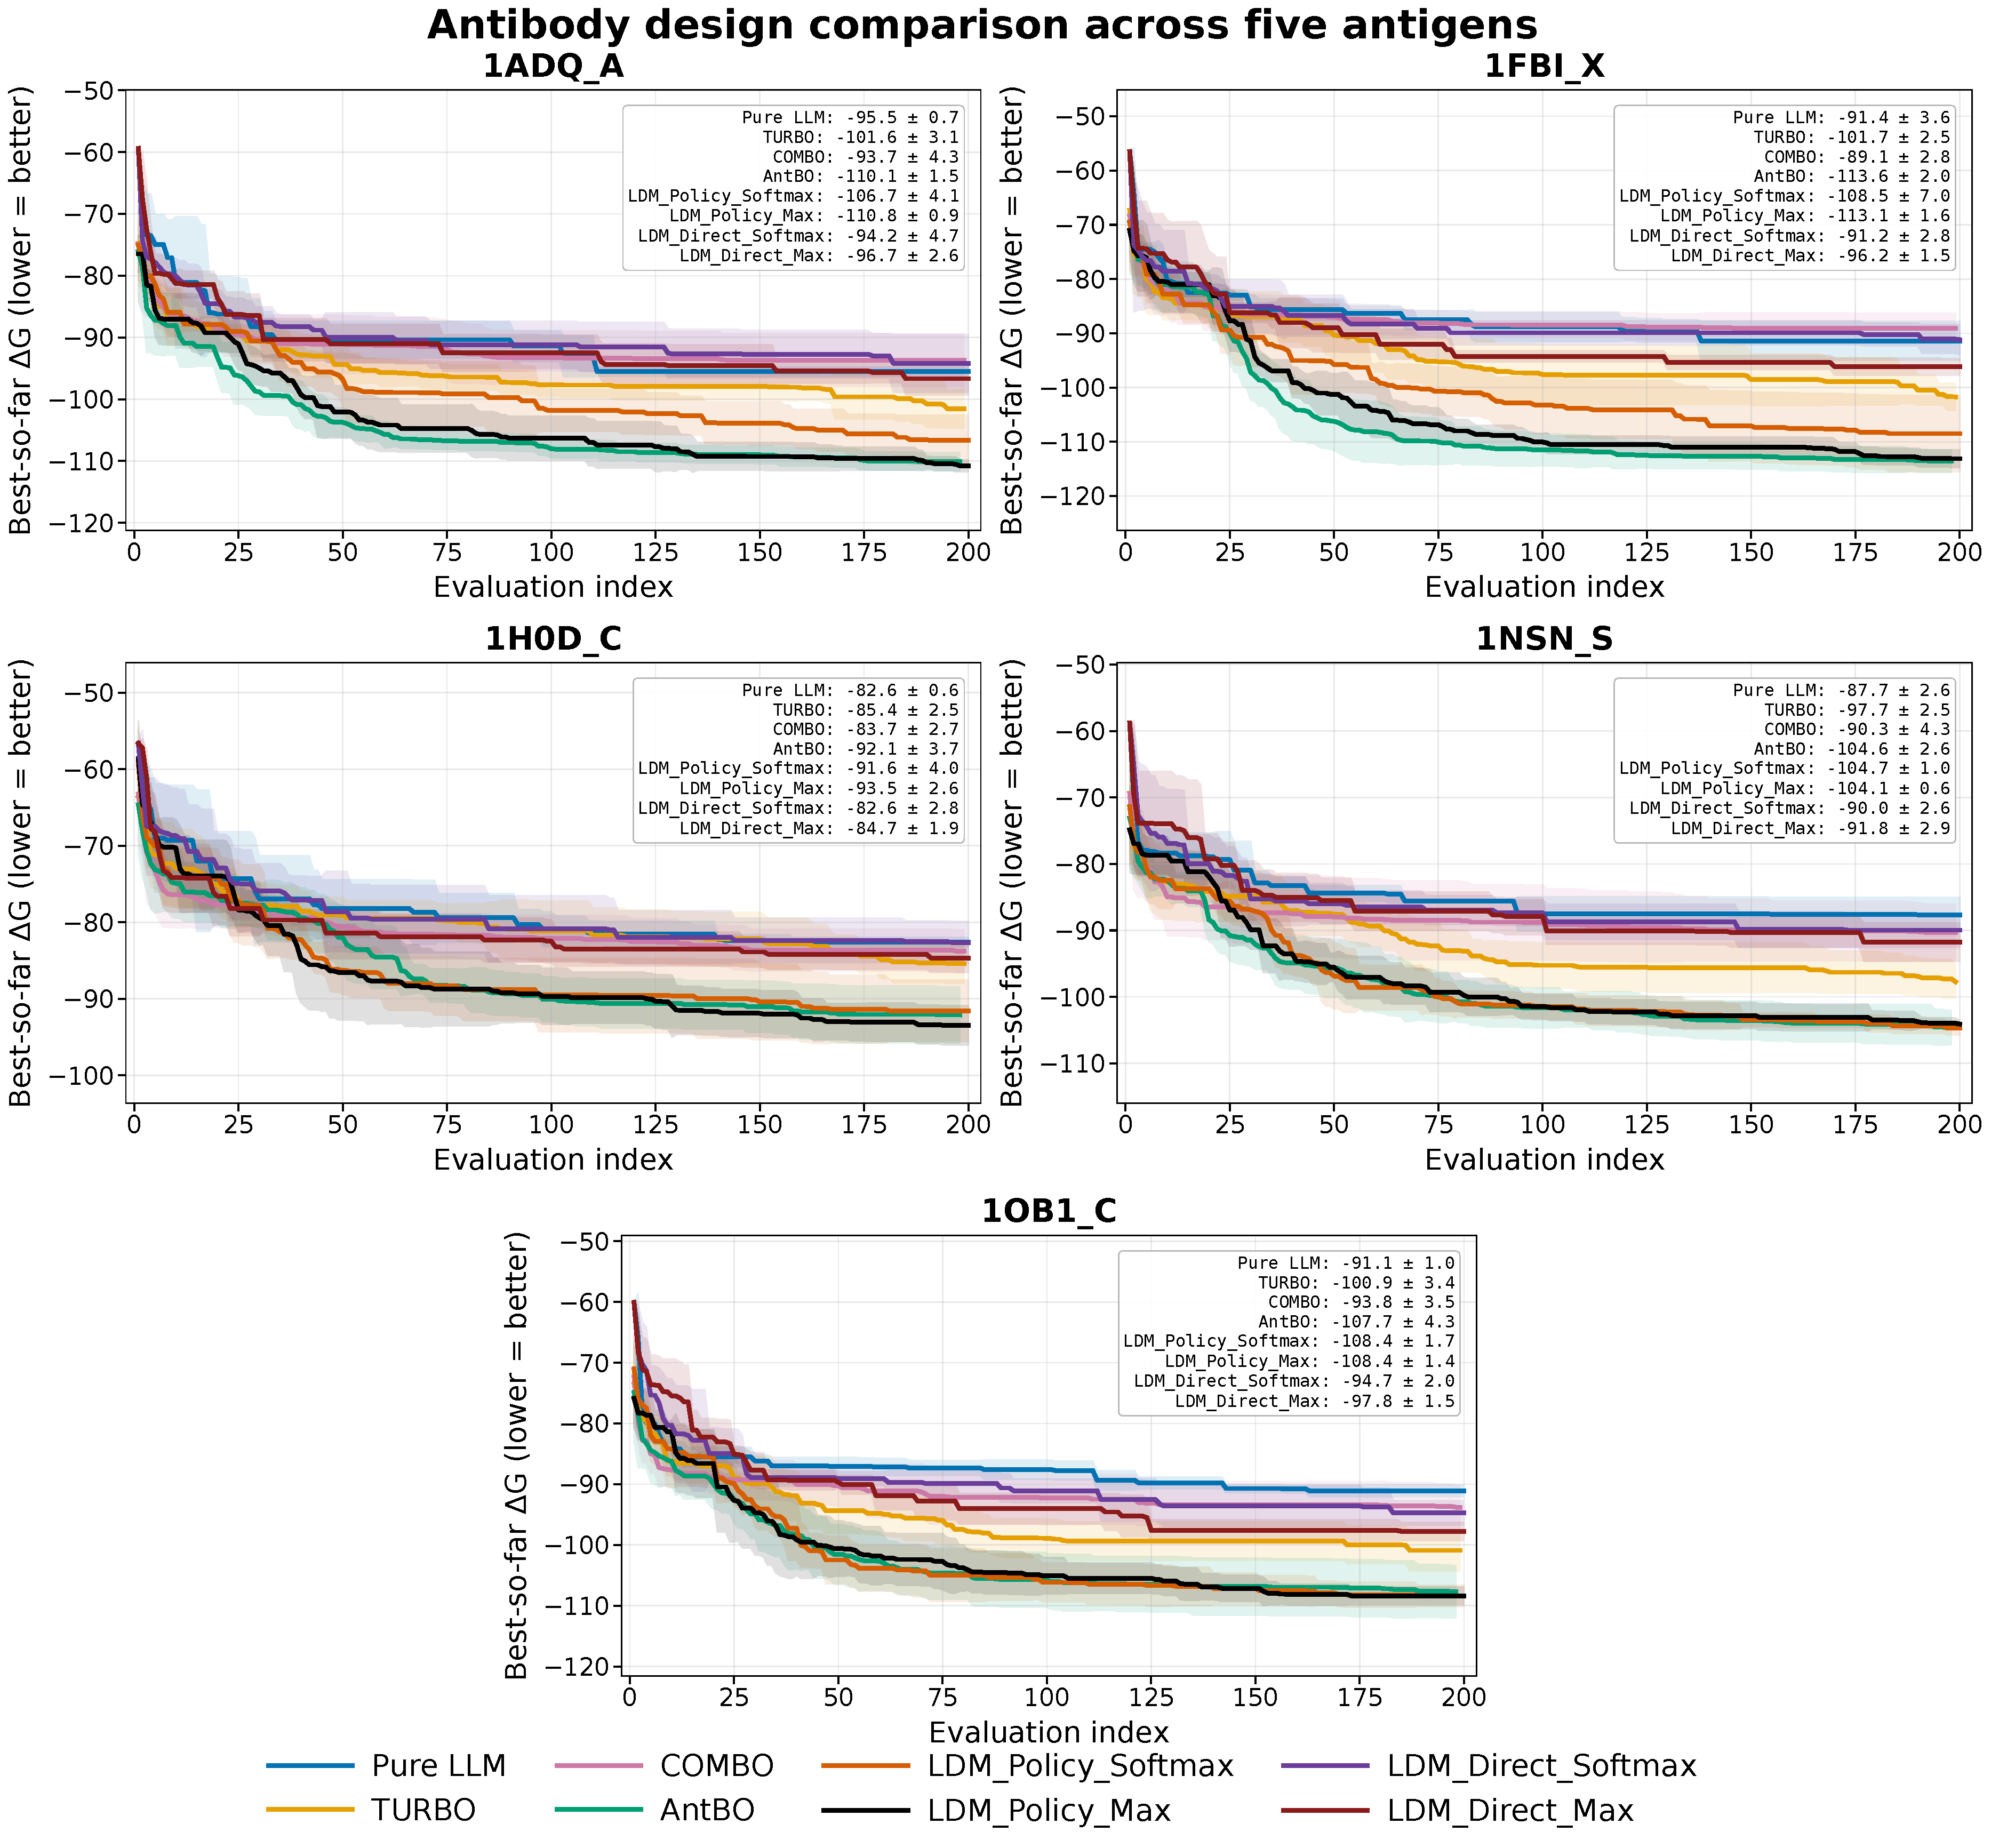
\includegraphics[width=1.0\linewidth]{figure/antibody_results.pdf}
\caption{Binding affinity performance across five antibody antigens. Axes: horizontal = number of sequence evaluations; vertical = best-so-far binding energy score (lower values indicate stronger binding). Curves correspond to all tested baselines and LDM variants.}
\label{fig:cs-antibody-results}
\end{figure}

Figure~\ref{fig:cs-antibody-results} compares all methods across the five protein targets. Policy-based LDM variants consistently outperform direct generation variants, achieving affinity levels comparable to AntBO, while Direct variants perform only marginally better than standalone LLMs.

Protein fitness landscapes are sparse and rugged, restricting the utility of small batches of directly generated sequences; even post-hoc acquisition reweighting cannot recover promising candidates the LLM fails to propose. In contrast, policy-mode LDM uses the LLM to define search regions rather than final sequences, expanding the candidate pool without extra oracle calls. This separation of semantic search scope planning (LLM) and calibrated value filtering (Bayesian surrogate) yields broader, more effective exploration of sequence neighbourhoods.

\begin{figure}[h!]
\centering
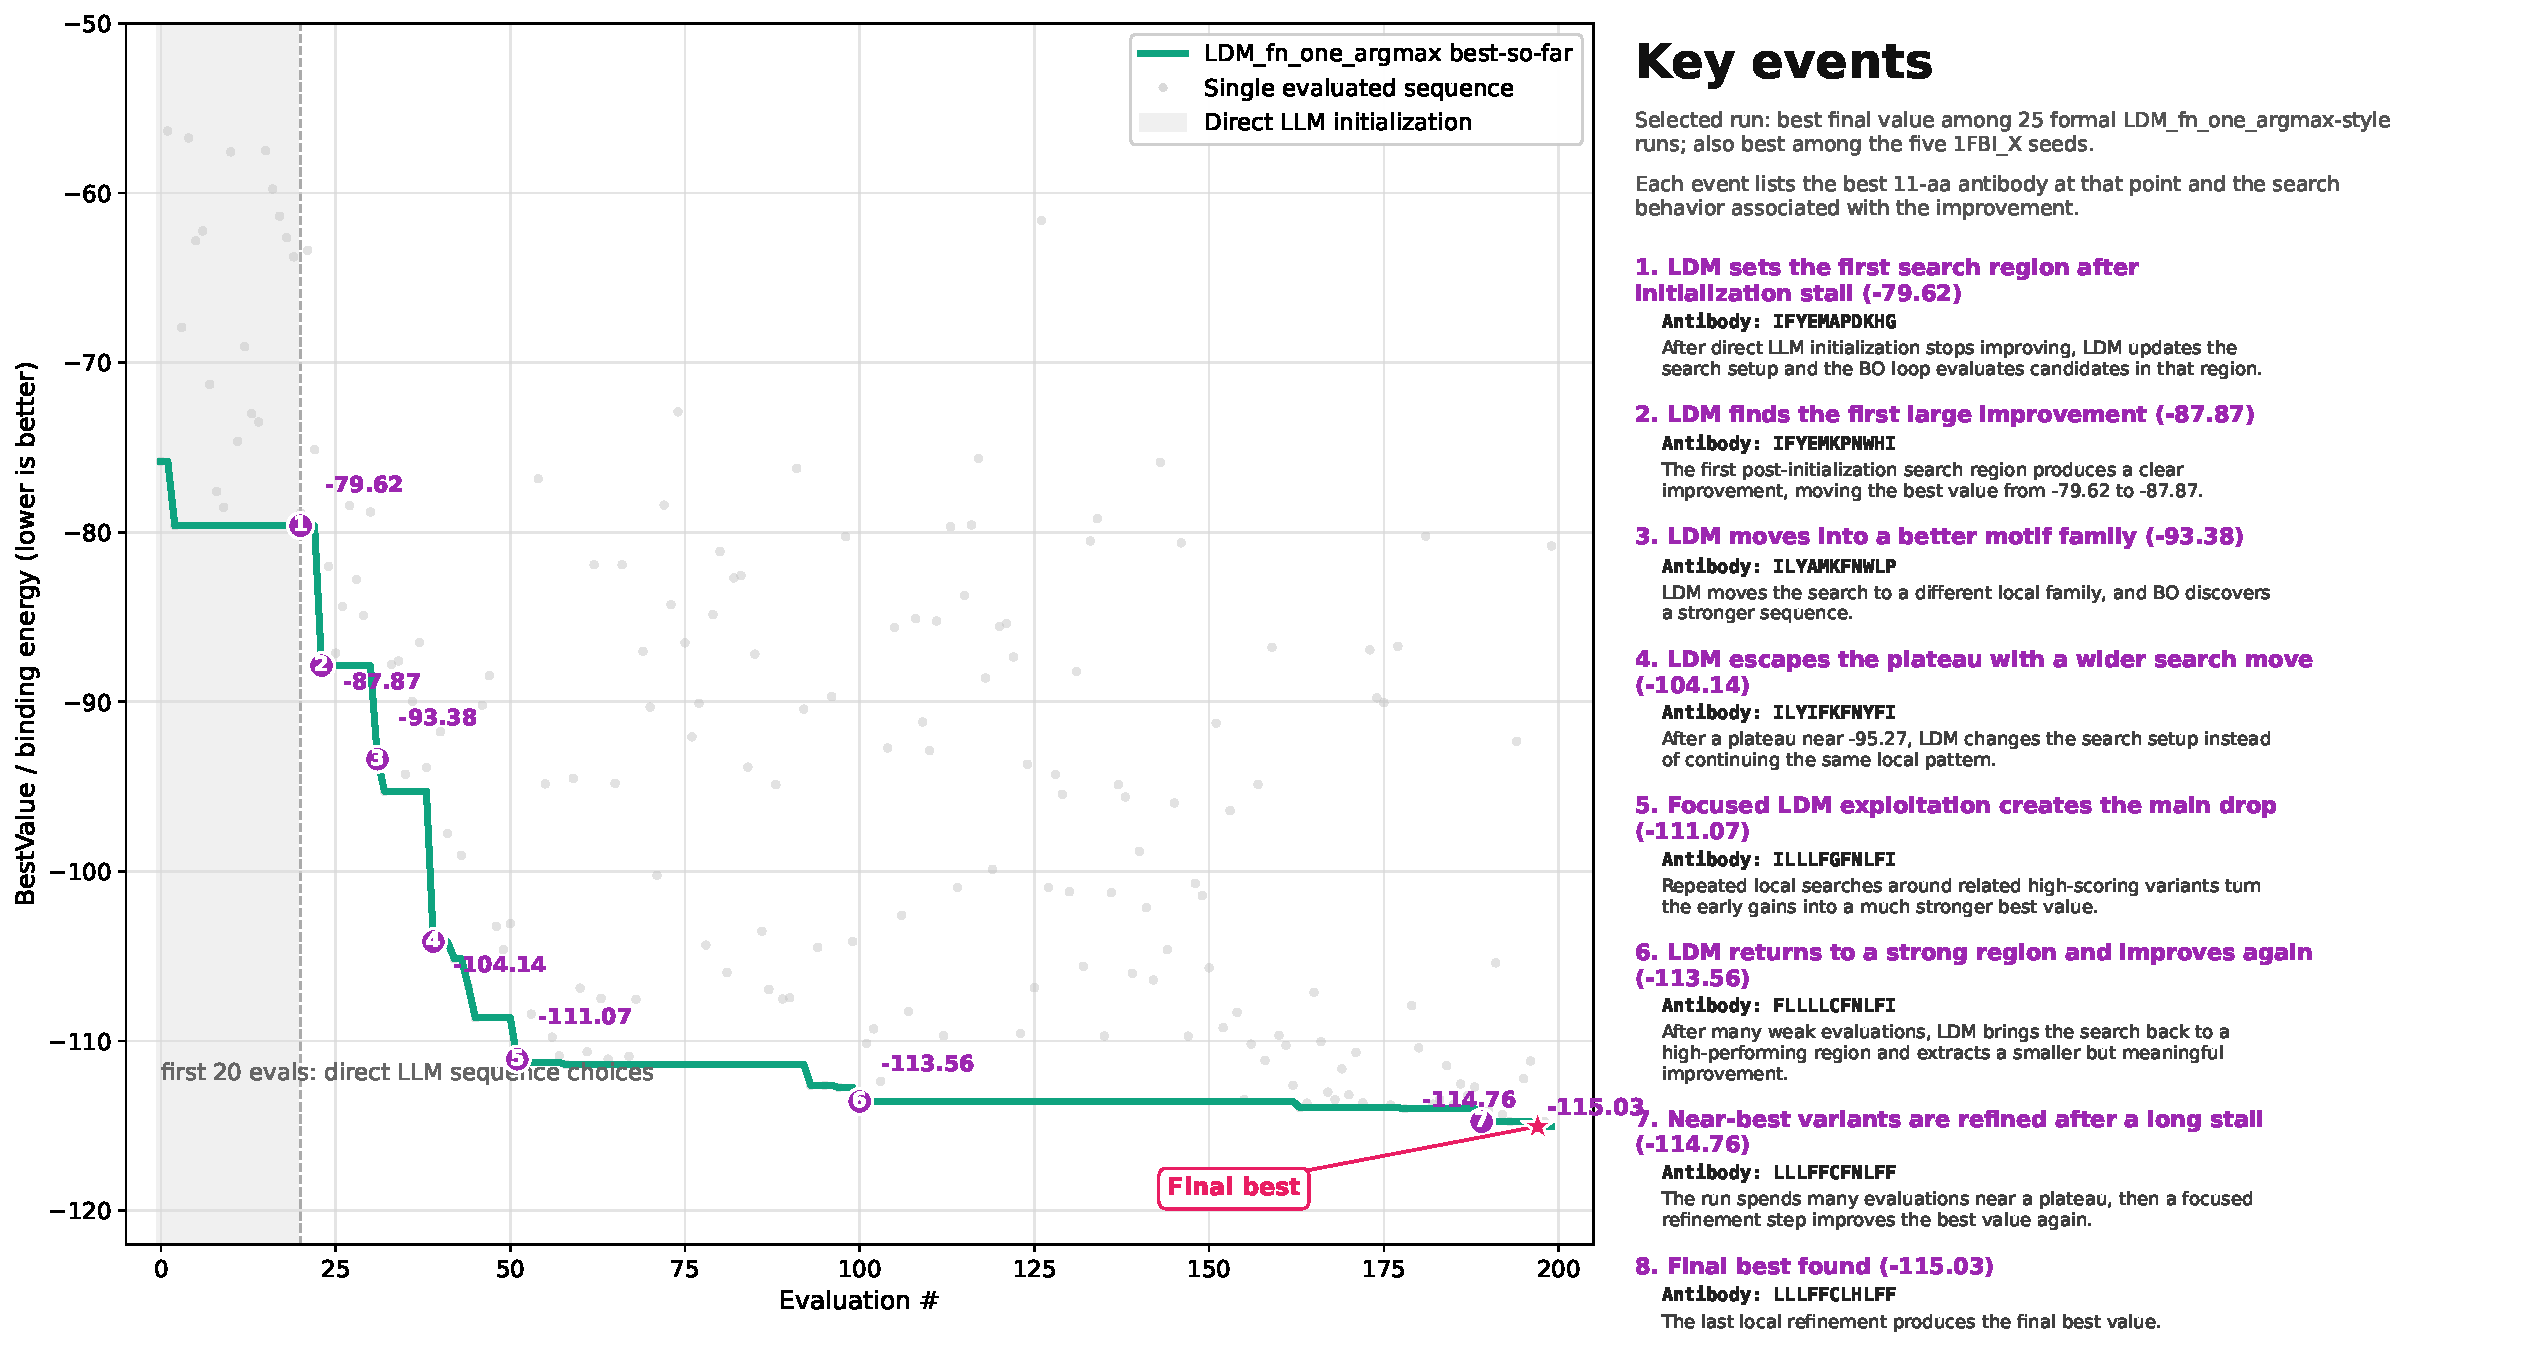
\includegraphics[width=0.95\linewidth]{figure/antibody_example_trajectory.pdf}
\caption{Optimisation trajectory of the top-performing LDM run on antigen 1FBI\_X. Horizontal axis counts evaluation rounds; vertical axis tracks the best binding energy found to date (lower = better). Step curve records global improvement milestones, with numbered markers highlighting major discovery events where the system introduces structurally novel sequence families after local plateaus.}
\label{fig:antibody_trajectory}
\end{figure}

Figure~\ref{fig:antibody_trajectory} visualises a representative LDM optimisation trajectory on the 1FBI\_X antigen, illustrating the core exploit–explore–discover cycle described in Section 2. Initial LLM sampling quickly hits a local performance ceiling; the LDM detects stagnation and triggers discovery steps to expand the sequence families under consideration. Each numbered marker denotes a discovery event that lifts the achievable performance ceiling, followed by phases of local refinement within the newly uncovered structural space.

% ============================================================
\subsection{Small-molecule drug discovery}
\label{sec:cs-molecule-results}

We select multi-objective small-molecule lead discovery as the third case study to test LDM’s handling of the \emph{unknown unknown} regime. Valid SMILES strings form an effectively unbounded chemical space with no clear global boundary, making full enumeration impossible. Standard multi-objective Bayesian optimisation (MOBO) with string kernels lacks strong structural priors and saturates rapidly. Auxiliary expansion tools such as ReaSyn only generate analogues around fixed seed molecules, limiting exploration to narrow local chemical neighbourhoods. This domain therefore benchmarks LDM’s unique capability to autonomously uncover entirely novel molecular scaffolds outside initial seed support.

Our multi-objective task optimises two conflicting rewards for the KRAS G12D target \citep{kumarOverviewKRASG12D2026}: AutoDock Vina \citep{trott2010AutoDockVina} docking score (\(R_{\mathrm{Vina}}\), minimise) and neural-network binding activity (\(R_{\mathrm{act}}\), maximise). We quantify performance via the hypervolume of the Pareto front, with a fixed reference point across all experiments and a total evaluation budget of 80 iterations.

\subsubsection{Experimental settings}

Independent Gaussian Process surrogates are fitted for each reward dimension, with the subsequence string kernel measuring SMILES structural similarity. Expected Hypervolume Improvement (EHVI) serves as the multi-objective acquisition function. Baselines include vanilla MOBO and random search. We evaluate two LDM instantiations sharing the same tilted sampling pipeline but differing in candidate pool construction:
\begin{enumerate}
    \item \textbf{Direct-Softmax}: The LLM generates large parallel batches of 128 raw SMILES candidates for acquisition-weighted resampling.
    \item \textbf{ReaSyn-Softmax}: The LLM outputs a small set of seed SMILES, with ReaSyn generating local analogues to build the candidate pool before softmax selection.
\end{enumerate}

\subsubsection{Results}

\begin{figure}[h!]
\centering
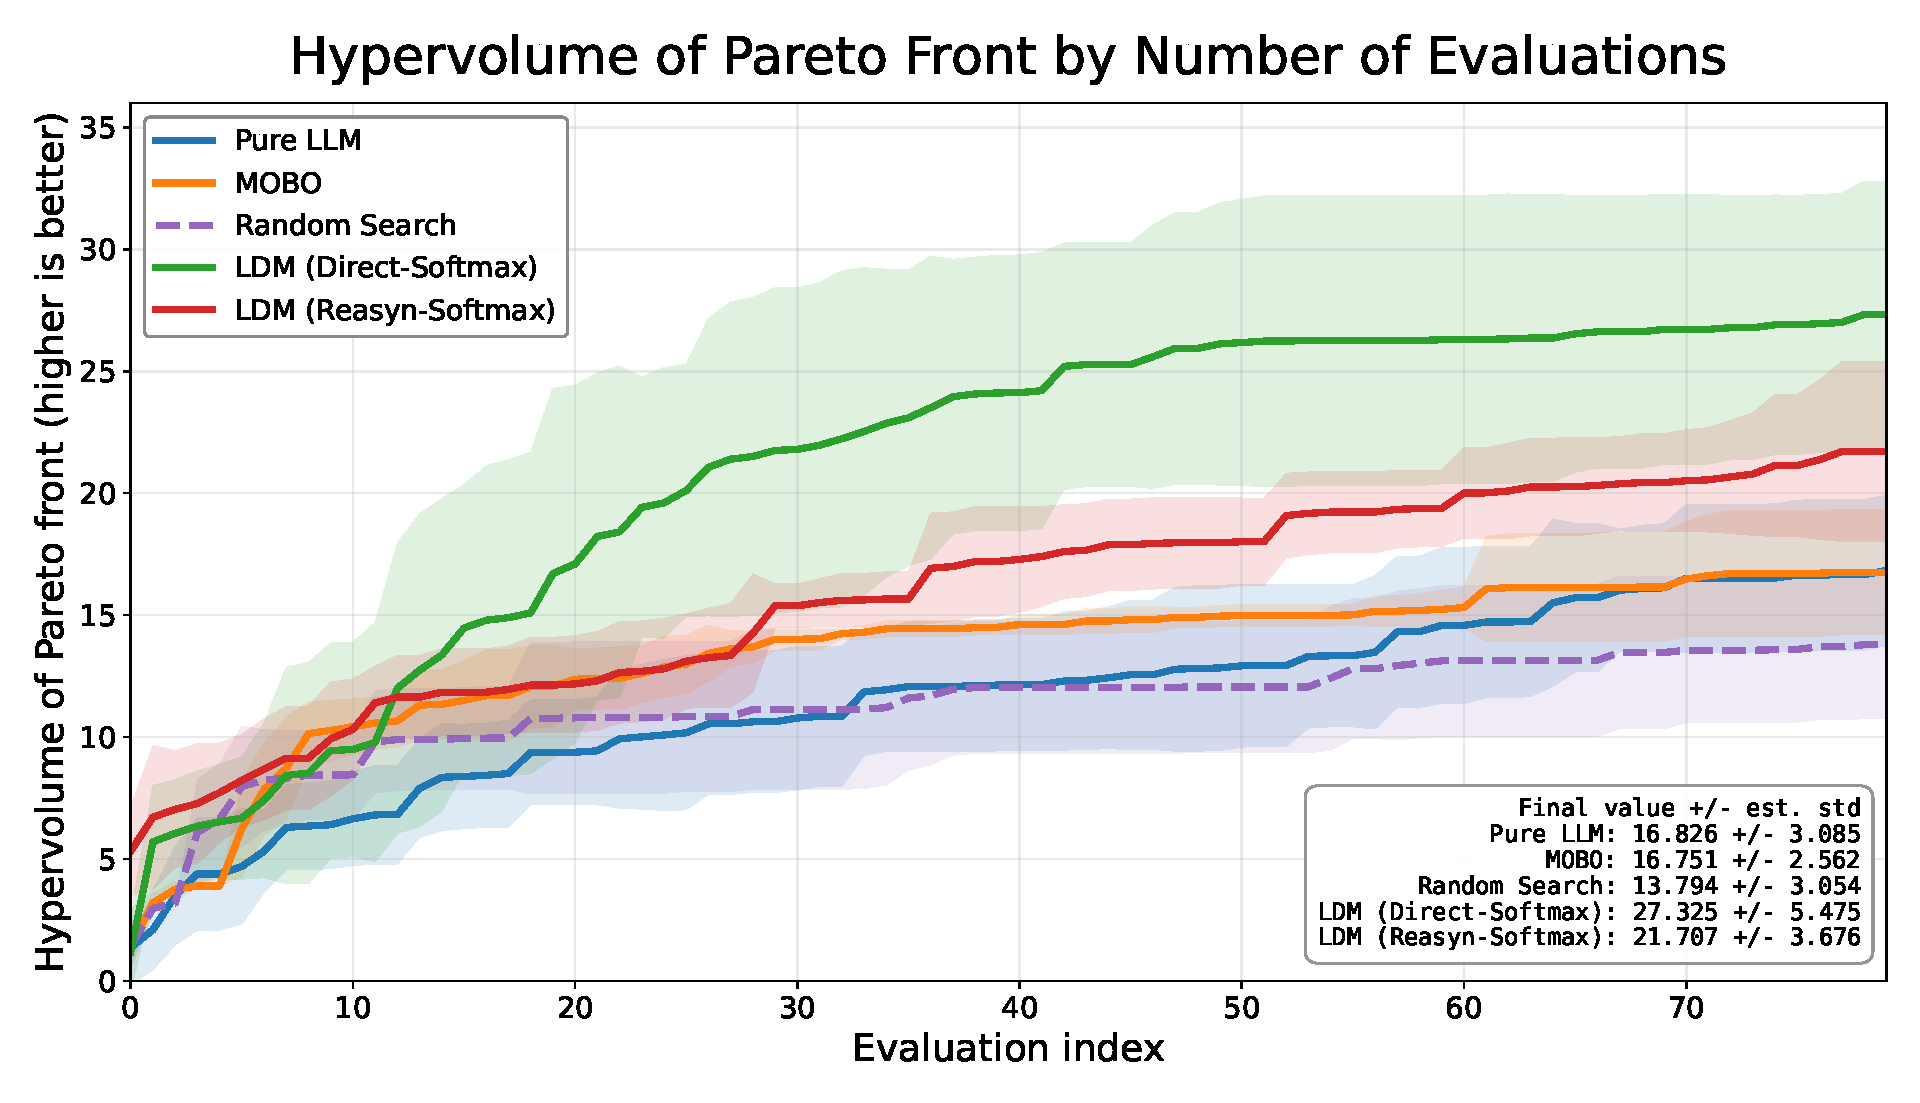
\includegraphics[width=0.6\linewidth]{figure/molecule_results.pdf}
\caption{Pareto hypervolume growth for molecular design. Horizontal axis = evaluation count; vertical axis = dominated hypervolume of the Pareto front (higher values denote better multi-objective trade-offs). Separate curves track performance of random search, standard MOBO, and the two LDM variants.}
\label{fig:cs-molecule-results}
\end{figure}

Figure~\ref{fig:cs-molecule-results} shows that both LDM variants outperform all baselines by a substantial margin, with Direct-Softmax delivering the strongest hypervolume gains. Conventional MOBO plateaus after roughly 40 evaluations, trapped within limited chemical regions, while direct LLM generation sustains steady front expansion across the full budget.

The performance gap between the two LDM variants arises from a breadth–synthesizability trade-off. General-purpose LLMs carry broad pre-training knowledge of diverse SMILES structures; large-batch direct generation unlocks wider scaffold exploration. ReaSyn’s local analogue generation improves synthetic tractability but restricts structural diversity, slowing Pareto expansion for early-stage lead discovery where novel scaffolds are prioritised.

\begin{figure}[h!]
\centering
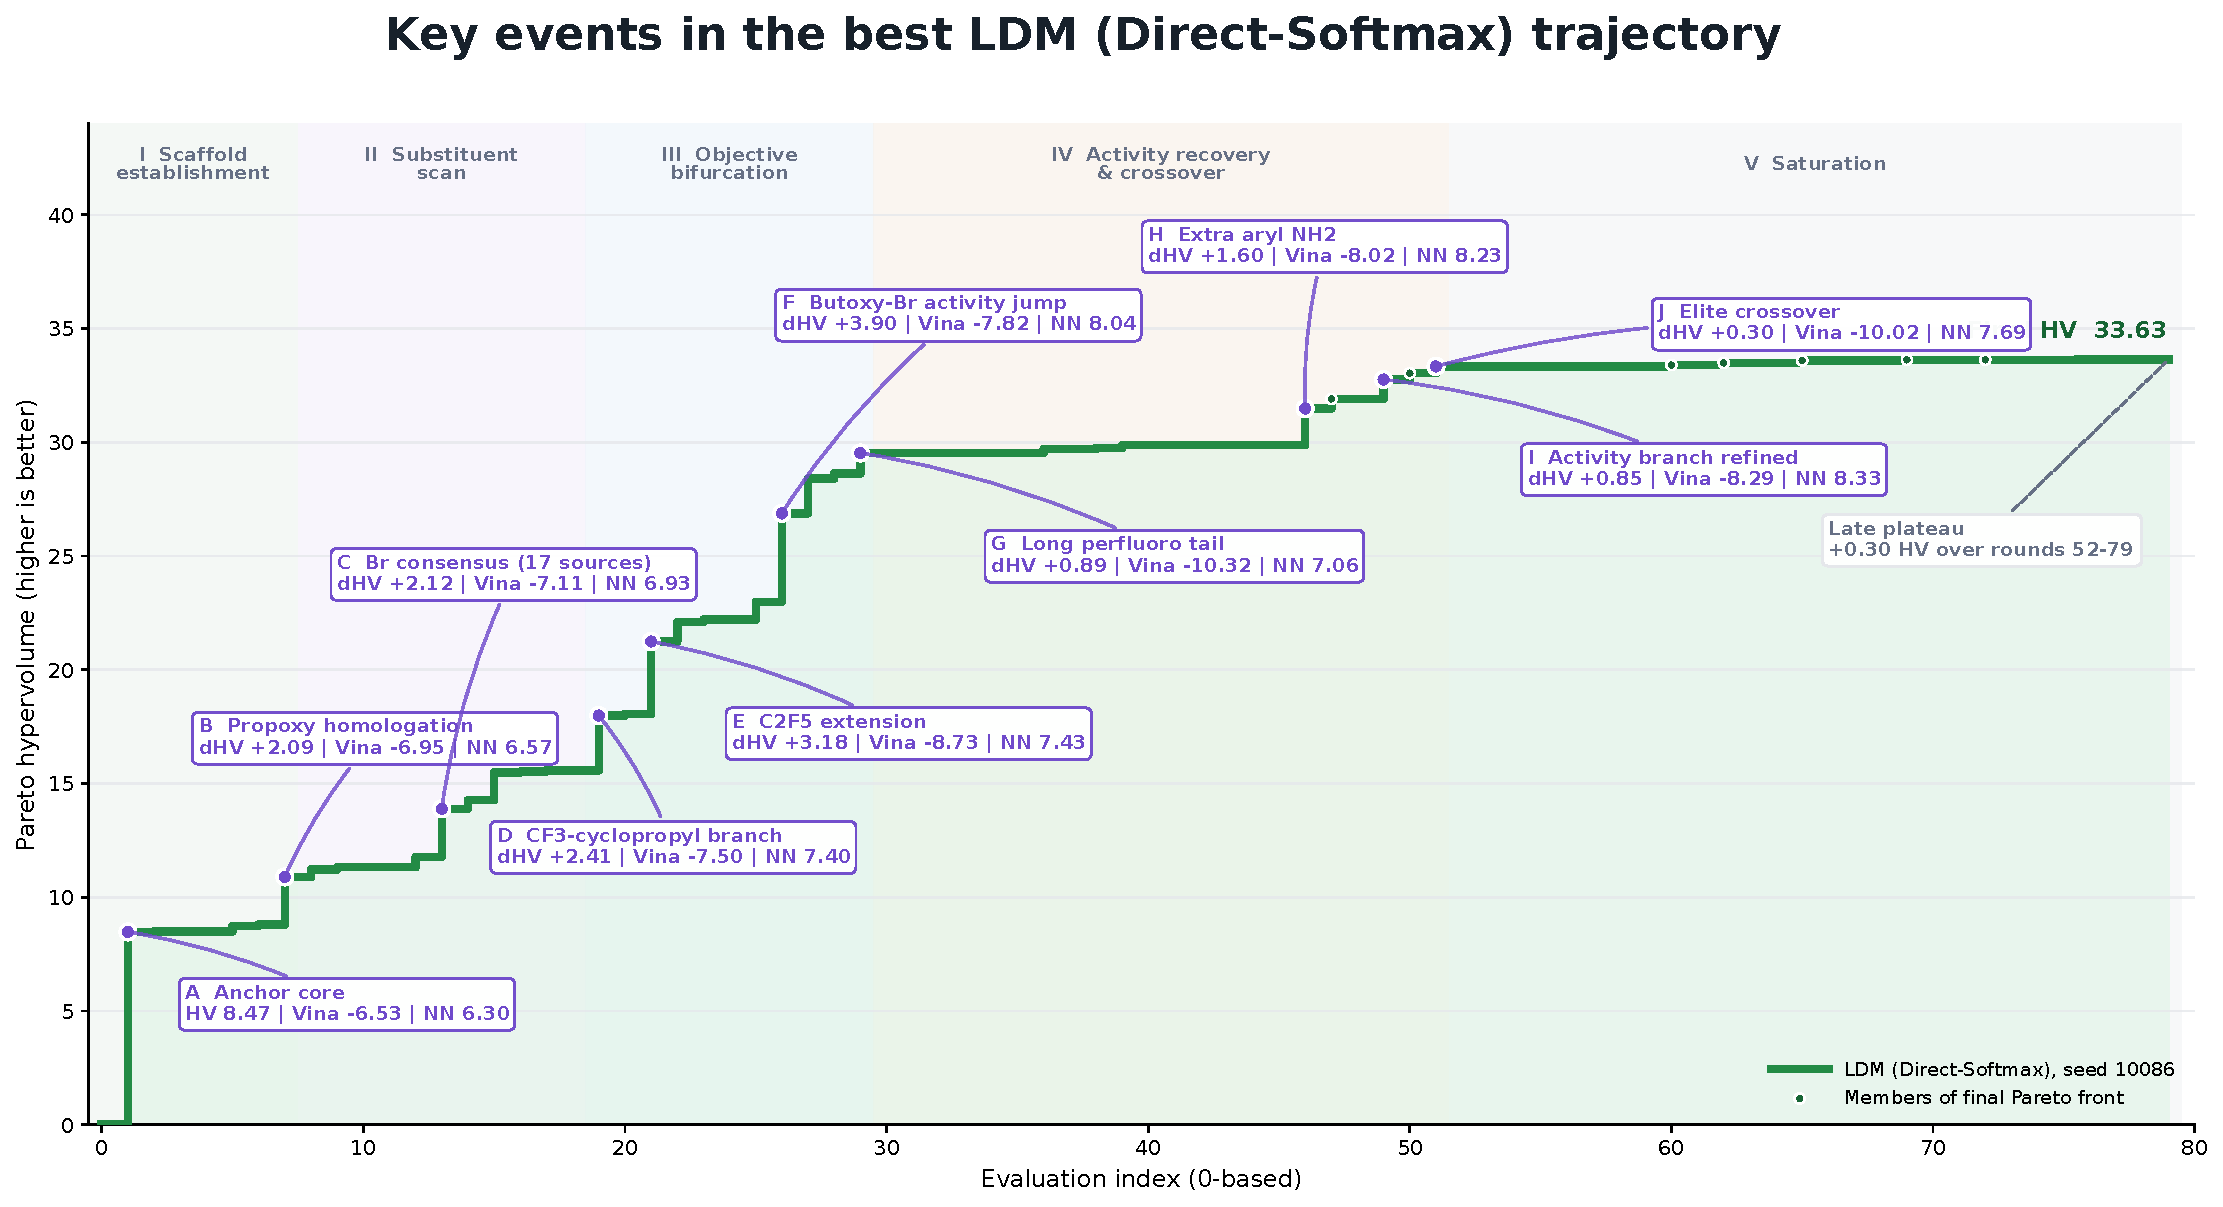
\includegraphics[width=1.0\linewidth]{figure/molecule_example_trajectory.pdf}
\caption{Key milestone events along a Direct-Softmax molecular optimisation trajectory. X-axis counts evaluation steps; Y-axis plots cumulative Pareto hypervolume (higher = better). Step curve tracks global front improvements, with labelled markers denoting structural discovery events that open new families of active molecules. Shaded bands partition the optimisation into five sequential search phases. In each text box, \texttt{HV} represents Hyper-Volumn, \texttt{Vina} represents the score of Autodock Vina, and \texttt{NN} represents the neural network as the oracle activity prediction.}
\label{fig:direct_softmax_key_events}
\end{figure}

\begin{figure}[h!]
\centering
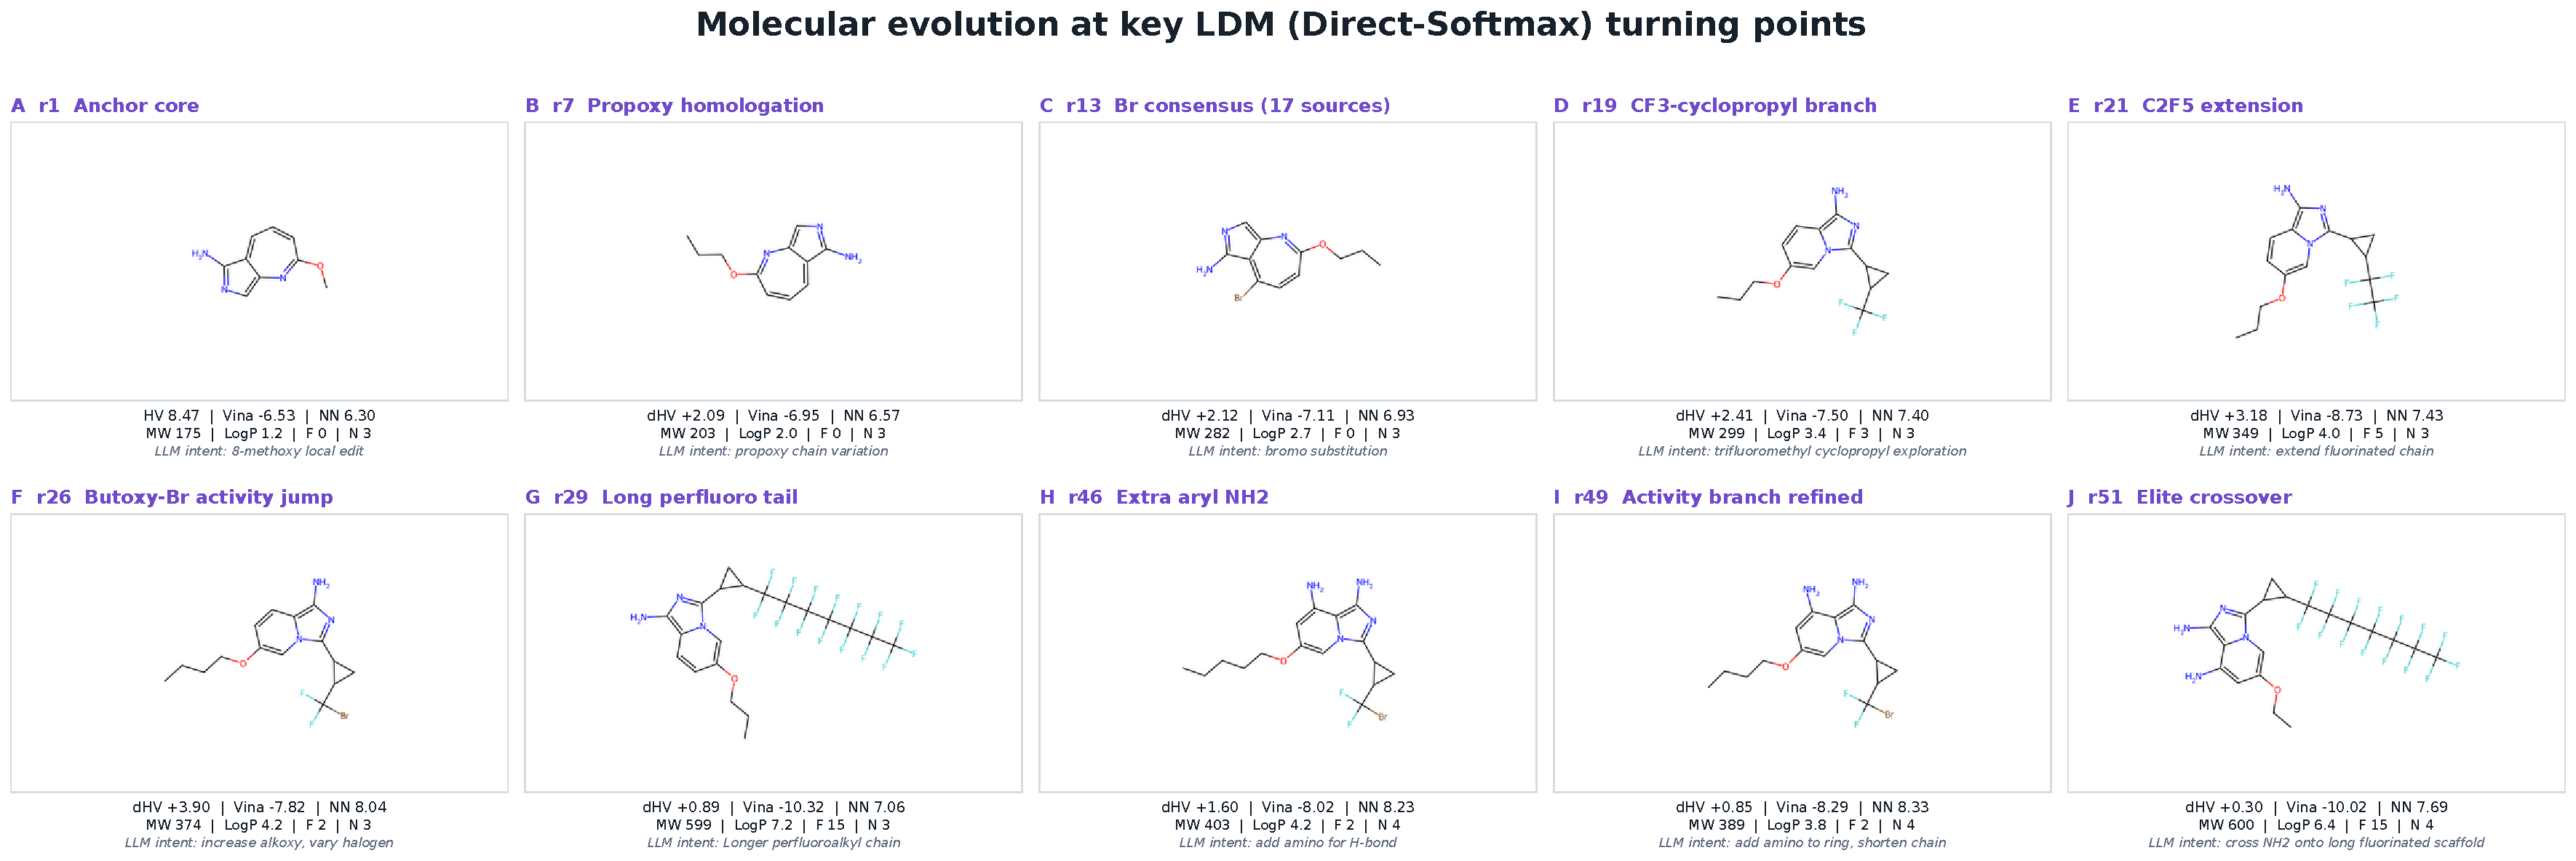
\includegraphics[width=1.0\linewidth]{figure/molecule_example_key_smiles.pdf}
\caption{Two-dimensional molecular structures corresponding to the ten core discovery milestones labelled in Figure~\ref{fig:direct_softmax_key_events}. Each structure is generated from canonical trajectory SMILES strings, arranged in chronological order of discovery to visualise the evolution of core chemical scaffolds and functional group substitutions.}
\label{fig:direct_softmax_molecular_evolution}
\end{figure}

Figures~\ref{fig:direct_softmax_key_events} and~\ref{fig:direct_softmax_molecular_evolution} together illustrate a complete LDM discovery workflow for small molecules. The hypervolume curve partitions optimisation into distinct stages: initial scaffold identification, substituent screening, objective bifurcation into docking- and activity-focused chemotypes, cross-family feature recombination, and final fine-tuning. The structural plot tracks how the model iteratively uncovers unrelated molecular backbones, a capability absent from standard BO or seed-local expansion tools.

%==============================finetune exp

\subsection{Fine-Tuning Experiments}
\label{sec:finetune-experiments}

We evaluate discovery fine-tuning across three structured design domains: multi-turn program search in AutoResearch, combinatorial antibody CDRH3 design, and multi-objective molecular discovery. In every experiment, the fine-tuned proposer is placed inside the same acquisition-guided LDM loop as the base proposer. Fine-tuning therefore changes the proposal reservoir, whereas the online surrogate continues to provide value and uncertainty estimates from the current experimental history.

We compare action-only discovery fine-tuning with reasoning-augmented fine-tuning. The latter trains the proposer to generate a surrogate-grounded research-progress rationale before emitting the candidate action.
\begin{figure*}[h!]
    \centering
    % Replace this path with the existing appendix path once located.
    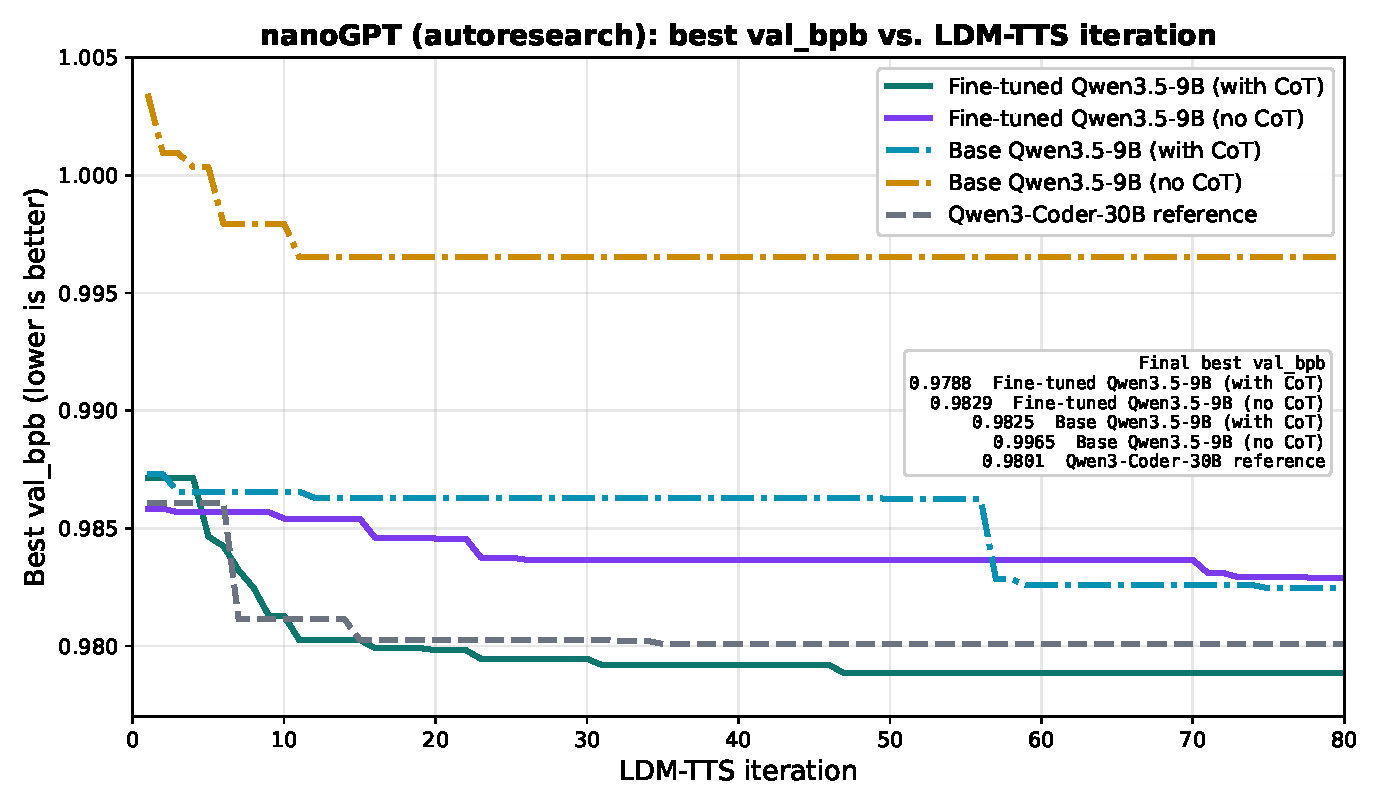
\includegraphics[width=0.82\textwidth]{figure/nanogpt_finetune_cot.pdf}
    \caption{\textbf{Reasoning-augmentation ablation on AutoResearch.} Best validation bits-per-byte (lower is better) versus LDM-TTS iteration inside an identical acquisition-guided loop, comparing fine-tuned and base proposers with and without reasoning augmentation and the Qwen3-Coder-30B reference.}
    \label{fig:finetune-autoresearch}
\end{figure*}

\subsubsection{AutoResearch}

We first study fine-tuning in AutoResearch, where an agent repeatedly edits a persistent training program and evaluates each proposal through a fixed-budget nanoGPT training run. This setting requires the model to interpret an evolving experiment ledger, recognize performance plateaus, and propose changes that test new program mechanisms.

Figure~\ref{fig:finetune-autoresearch} compares fine-tuned and base Qwen3.5-9B proposers over 80 LDM-TTS iterations. The reasoning-augmented fine-tuned model achieves the best validation performance, reaching $\mathrm{val\_bpb}=0.9788$, lower than the Qwen3-Coder-30B reference at $0.9801$. Fine-tuning without reasoning reaches $0.9829$, the base model with reasoning reaches $0.9825$, and the base model without reasoning stalls at $0.9965$. These results show that fine-tuning improves the program-search reservoir and that the explicit research-progress trace further helps the model escape local program families.

\subsubsection{Antibody CDRH3 Design}

We next evaluate antibody CDRH3 design, where the proposer searches a sparse and rugged sequence space under a limited binding-energy evaluation budget. We compare fine-tuned and base Qwen3.5-9B models with and without reasoning augmentation across five antigens. All variants use the same acquisition-guided LDM loop with expected-improvement acquisition and the same parallel evaluation budget.

Figure~\ref{fig:finetune-antibody} shows that fine-tuning improves over the corresponding base proposer across the five antigens. Both fine-tuned variants achieve lower binding energies than the base models, while the reasoning-augmented fine-tuned model obtains the lowest average binding energy among the four configurations. This result indicates that the distilled policy improves sequence-family proposals even in a large discrete design space.

\begin{figure*}[h!]
    \centering
    % Replace this path with the existing appendix path once located.
    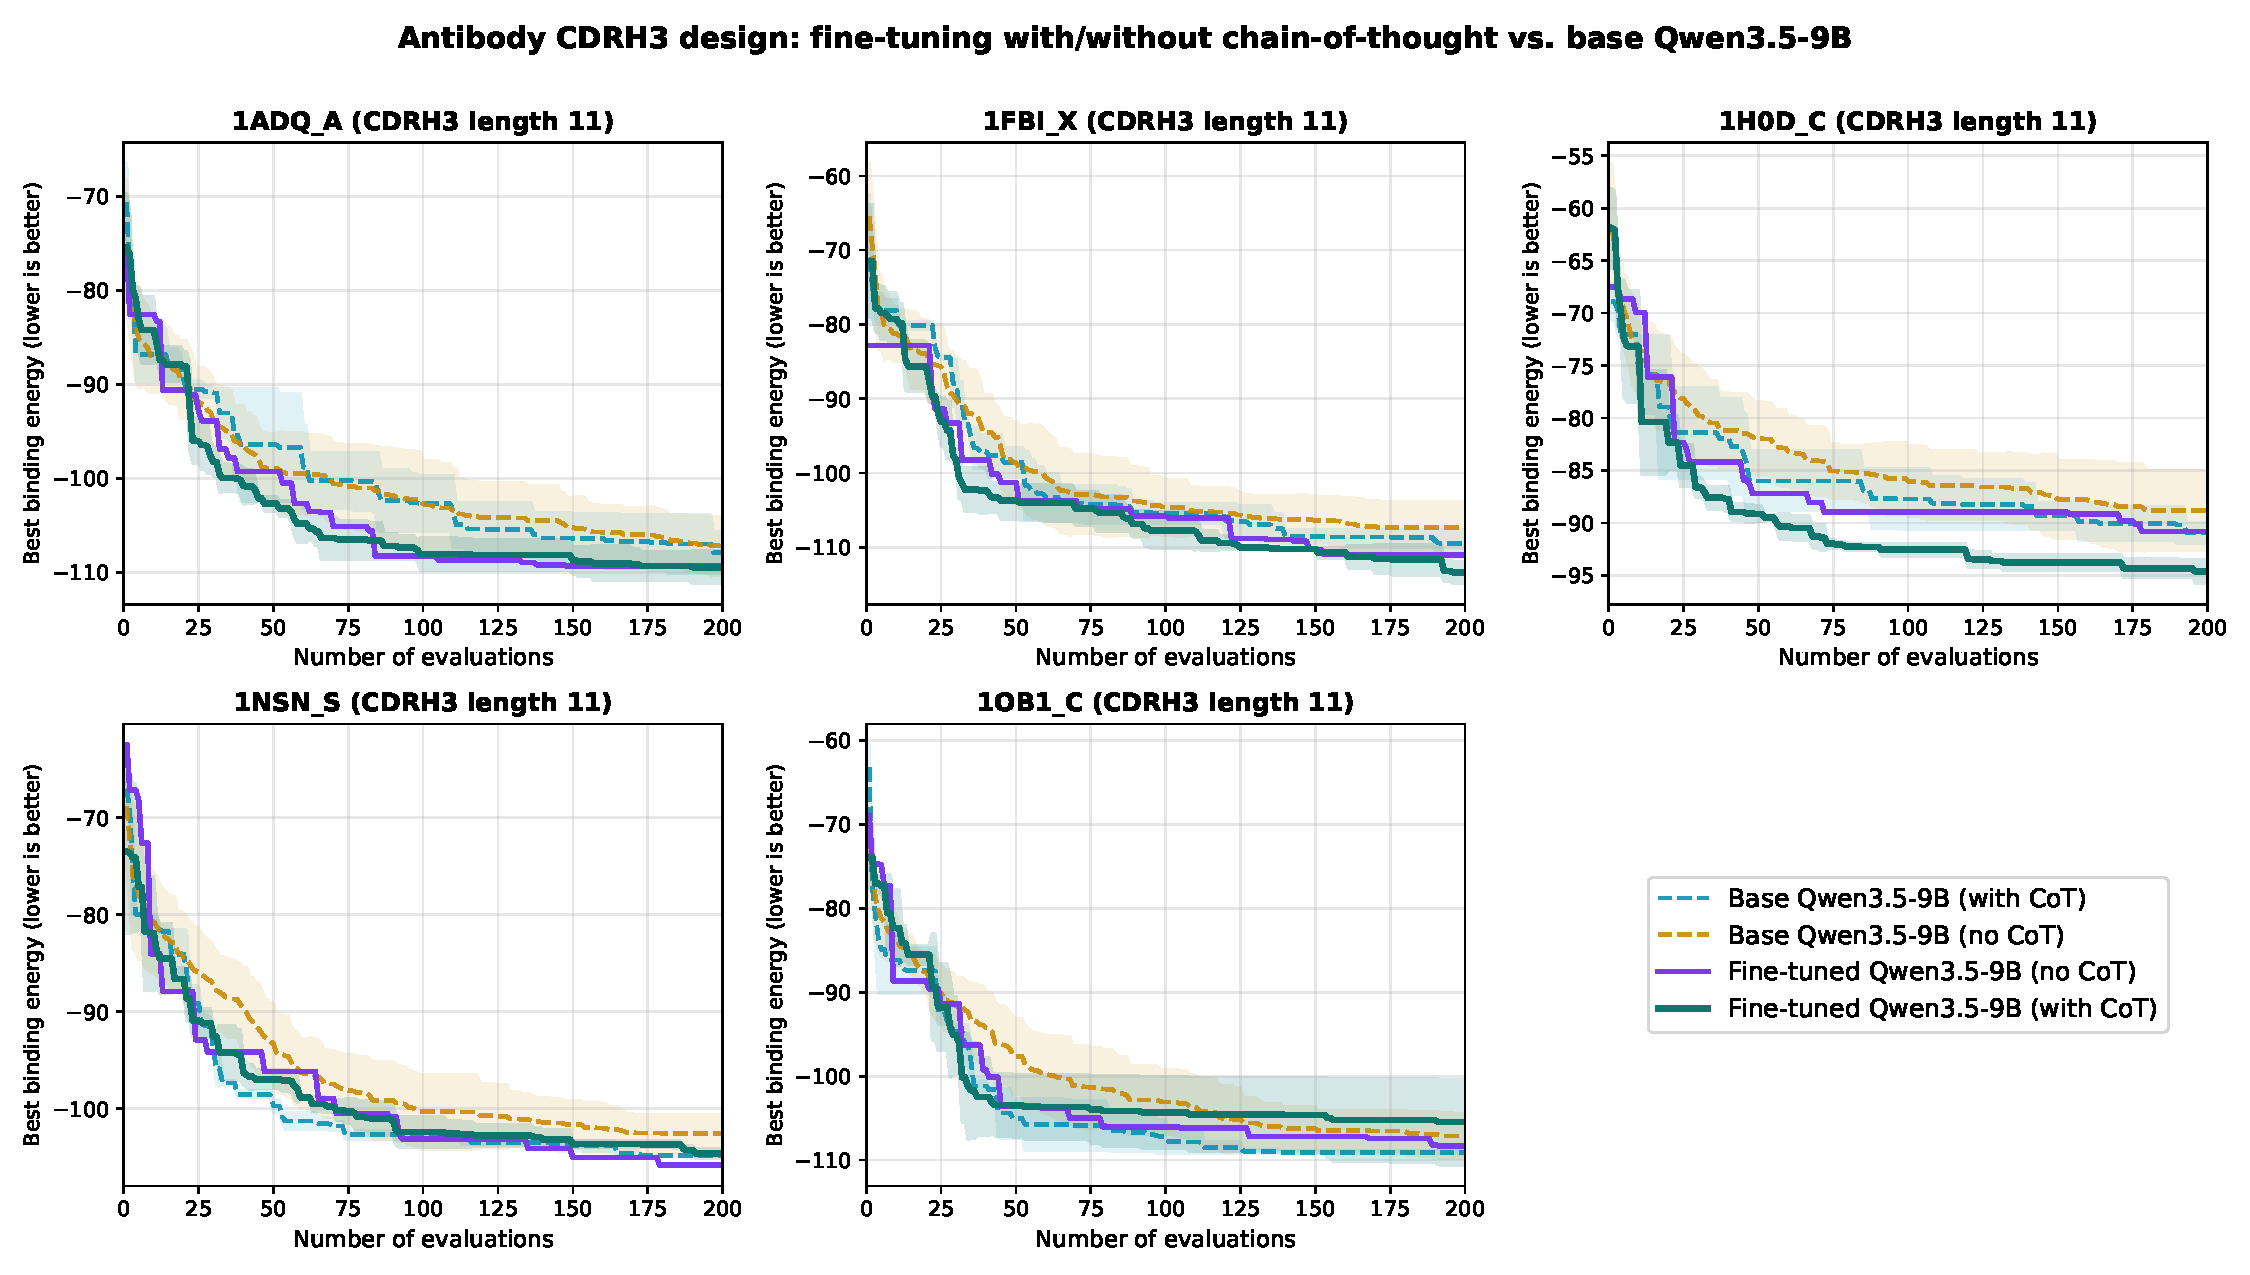
\includegraphics[width=0.94\textwidth]{figure/protein_finetune_cot.pdf}
    \caption{\textbf{Discovery fine-tuning for antibody CDRH3 design.} Best Absolut! binding energy, lower is better, versus the number of evaluations across five antigens. Fine-tuned Qwen3.5-9B variants with and without reasoning augmentation are compared with their corresponding base proposers in the same acquisition-guided LDM loop. Shaded bands denote mean $\pm$ standard deviation across available seeds.}
    \label{fig:finetune-antibody}
\end{figure*}

\subsubsection{Multi-objective Small-Molecule Discovery}

Finally, we evaluate cross-task transfer on the KRAS G12D molecular-design task. The task jointly optimizes docking and neural activity, and performance is measured by best-so-far Pareto-front hypervolume over 80 expensive evaluations.

Figure~\ref{fig:finetune-molecule} compares five inference-time policies inside the same LDM loop. The reasoning-augmented fine-tuned Qwen3.5-9B model achieves the highest final hypervolume, $26.660 \pm 2.608$. It exceeds the same fine-tuned student without reasoning, $22.279 \pm 3.828$, and both DeepSeek V4 Flash teacher variants, which reach $24.548 \pm 3.589$ with reasoning and $23.582 \pm 2.832$ without reasoning. The untuned Qwen3.5-9B base proposer reaches $16.489 \pm 5.867$. The result shows that the distilled policy transfers beyond the source task and that reasoning augmentation substantially improves this transfer.

\begin{figure*}[h!]
    \centering
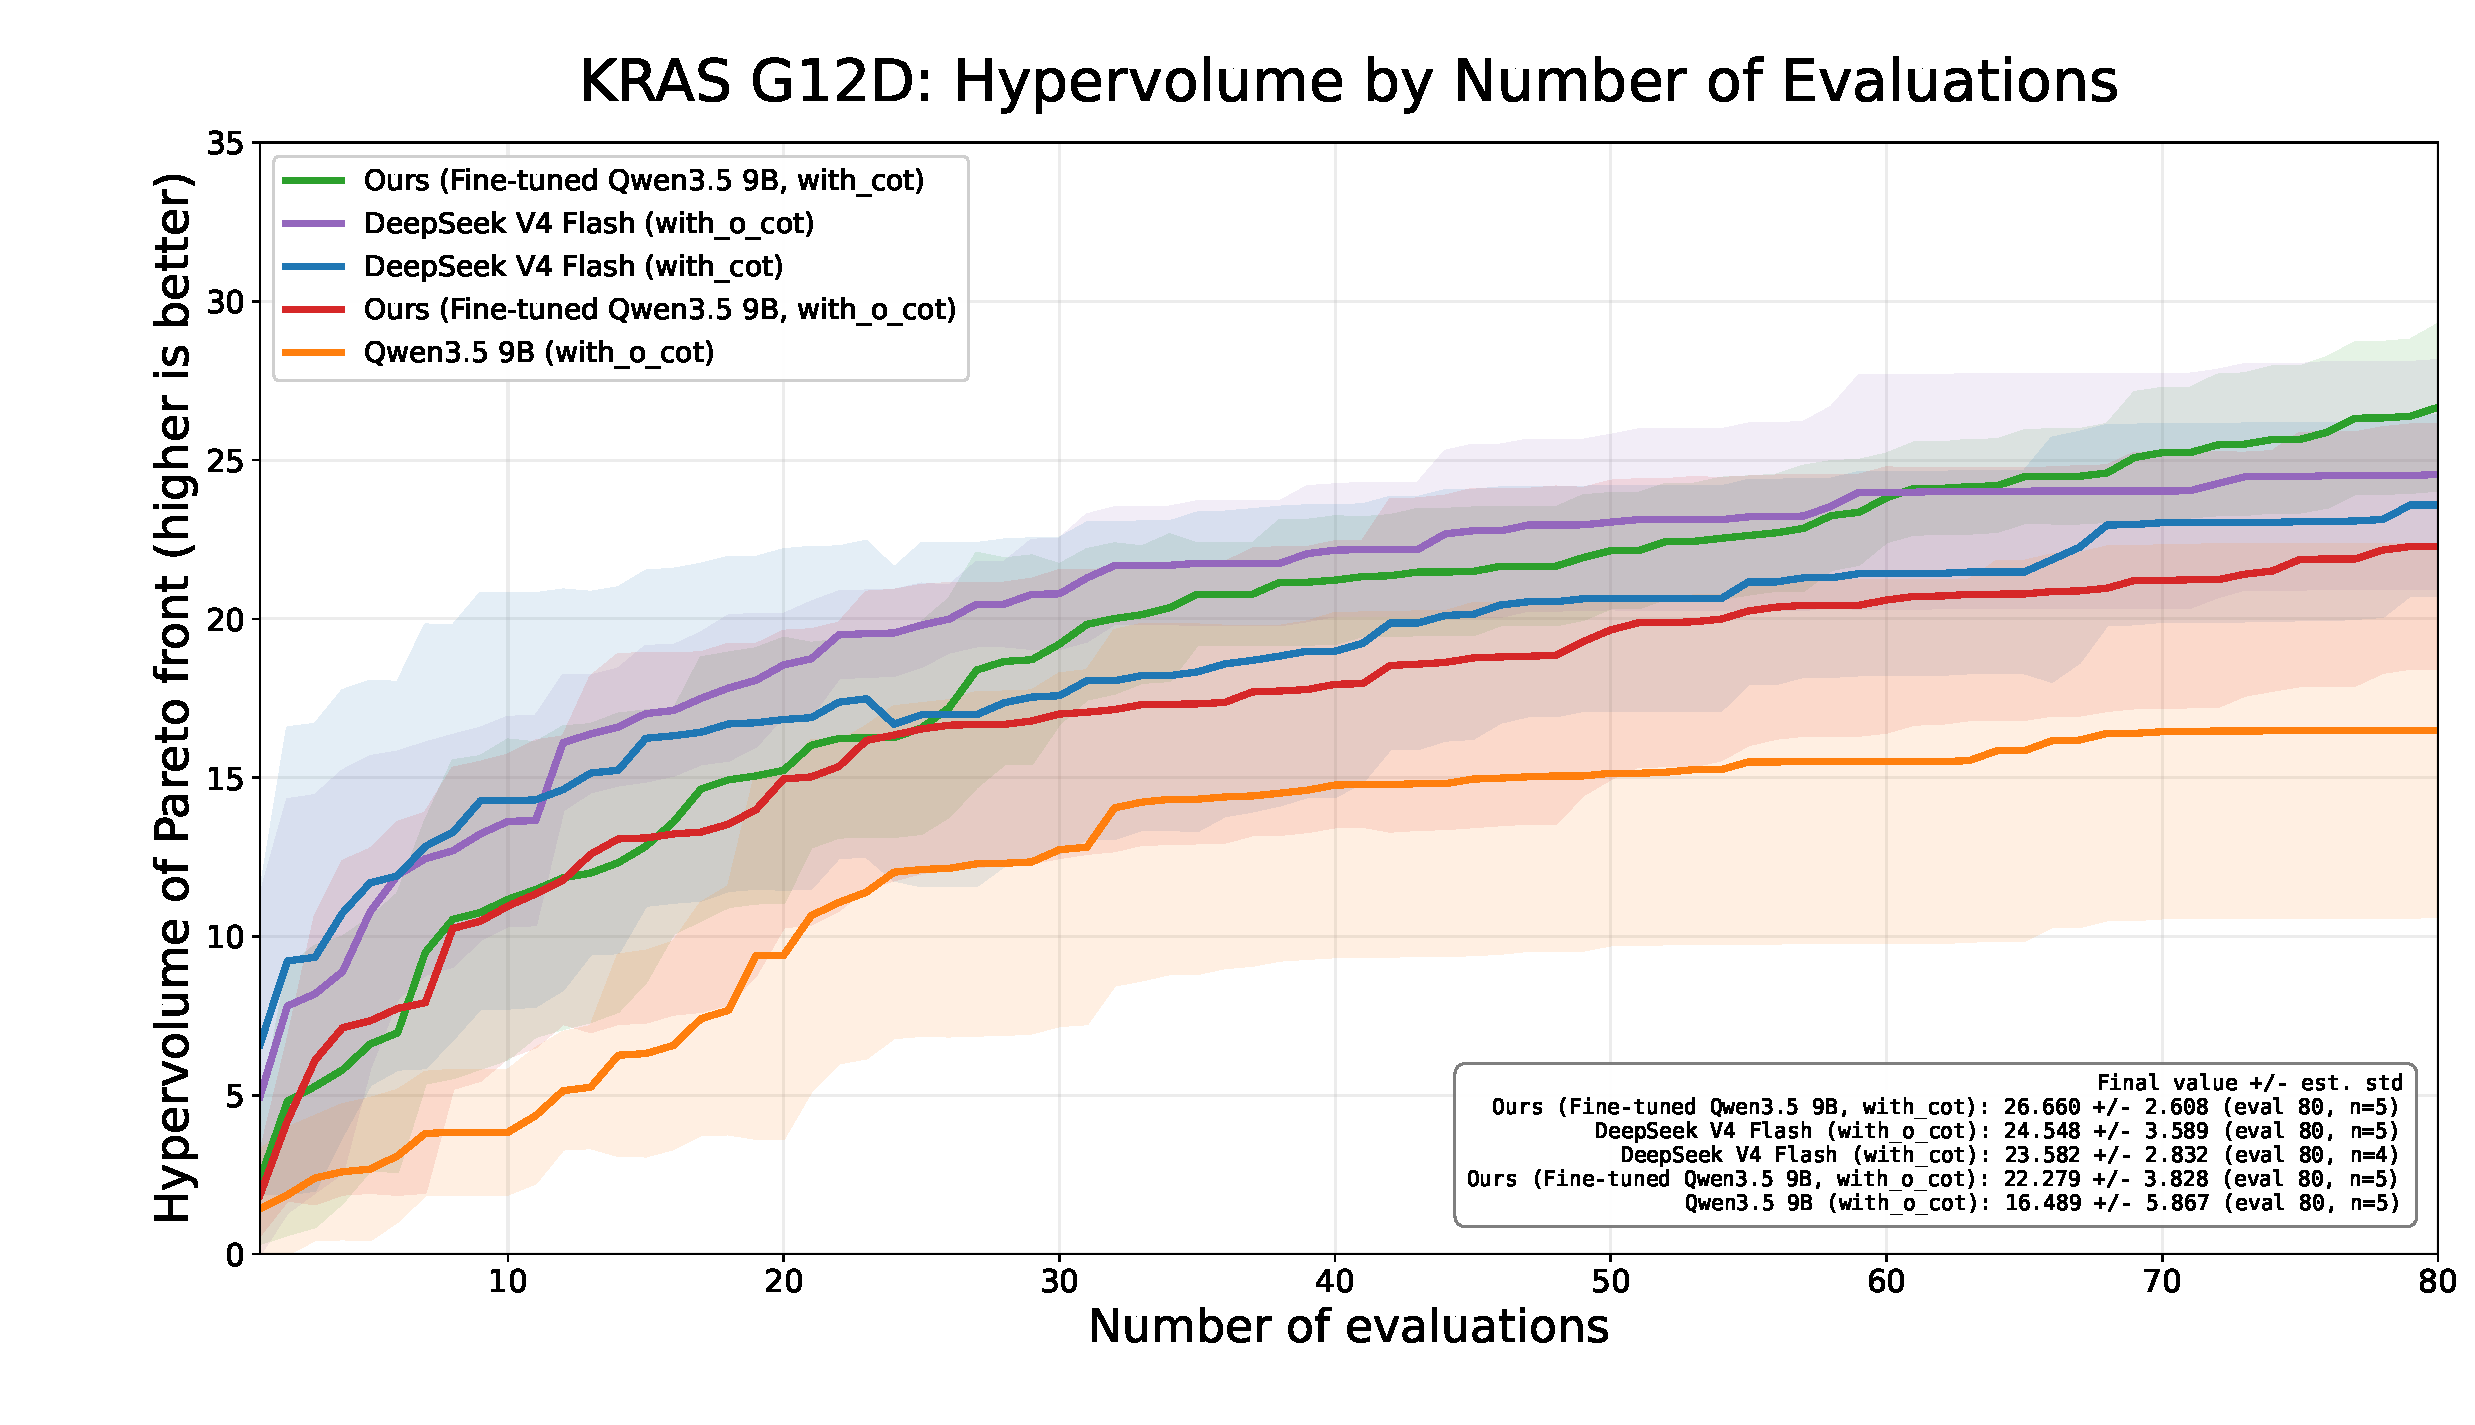
\includegraphics[width=0.82\textwidth]{figure/ldm_sft_small.pdf}
    \caption{\textbf{Fine-tuning with reasoning-augmented discovery data on KRAS G12D.} Best-so-far Pareto-front hypervolume (higher is better) versus the number of expensive evaluations, comparing fine-tuned and base proposers inside the same LDM loop. Shaded bands denote one standard deviation.}
    \label{fig:finetune-molecule}
\end{figure*}

Across programs, biological sequences, and molecules, fine-tuning improves the proposal reservoir within the online LDM loop. The gains are strongest when the model is trained to represent not only the next action but also the surrogate-grounded rationale for why that action advances scientific search.
% ============================================================
\subsection{Ablation Studies}
\label{sec:ablation-main}

The three case studies above have demonstrated the effectiveness of LDM in the spaces of programmes, biological sequences, and small molecules. In this section, we further conduct ablation experiments to investigate how LDM's gains depend on the test-time compute spent before each expensive evaluation, and how sensitive the policy is to its two temperature knobs $\alpha$ (LLM sampling temperature) and $\eta$ (acquisition tilt). Note that only partial ablation results are reported here; the remaining ablations results, including the pure LLM research loop on \texttt{autoresearch} with no BO value at all (\S\ref{app:abl-pure-llm}), the antibody CDRH3 hyperparameter sweep on $1\mathrm{NSN\_S}$, and the molecule and CDRH3 single-step budget sweeps (\S\ref{app:abl-ldm}), are reported in Appendix~\ref{app:ablation}.

\subsubsection{Test-time search scaling and acquisition functions}

We first ask whether LDM exhibits the same test-time scaling behaviour that motivates inference-time search in language-model reasoning \citep{snell2025scaling}, but in the harder setting where the value is an expensive scientific objective approximated by a surrogate. We keep the outer five-minute training budget fixed and vary only the cheap inner-loop budget of test-time search. The inner budget has two knobs: $N$ is the number of candidate \texttt{train.py} programs the LLM proposes at each outer iteration, and $H$ is the number of hypothesis/refinement branches each candidate is expanded into before the surrogate scores it; together they control the total acquisition-scored nodes per outer round, which we label \textsc{N$m$H$n$} so that \textsc{N4H4} scores $4 \times 4 = 16$ nodes per round and \textsc{N8H8} scores $8 \times 8 = 64$. We additionally vary whether the surrogate uses a fixed or dynamically expanded program-feature representation and which acquisition is used as the value (posterior mean only, EI, or an uncertainty-aware value).

\begin{figure}[htbp]
    \centering
    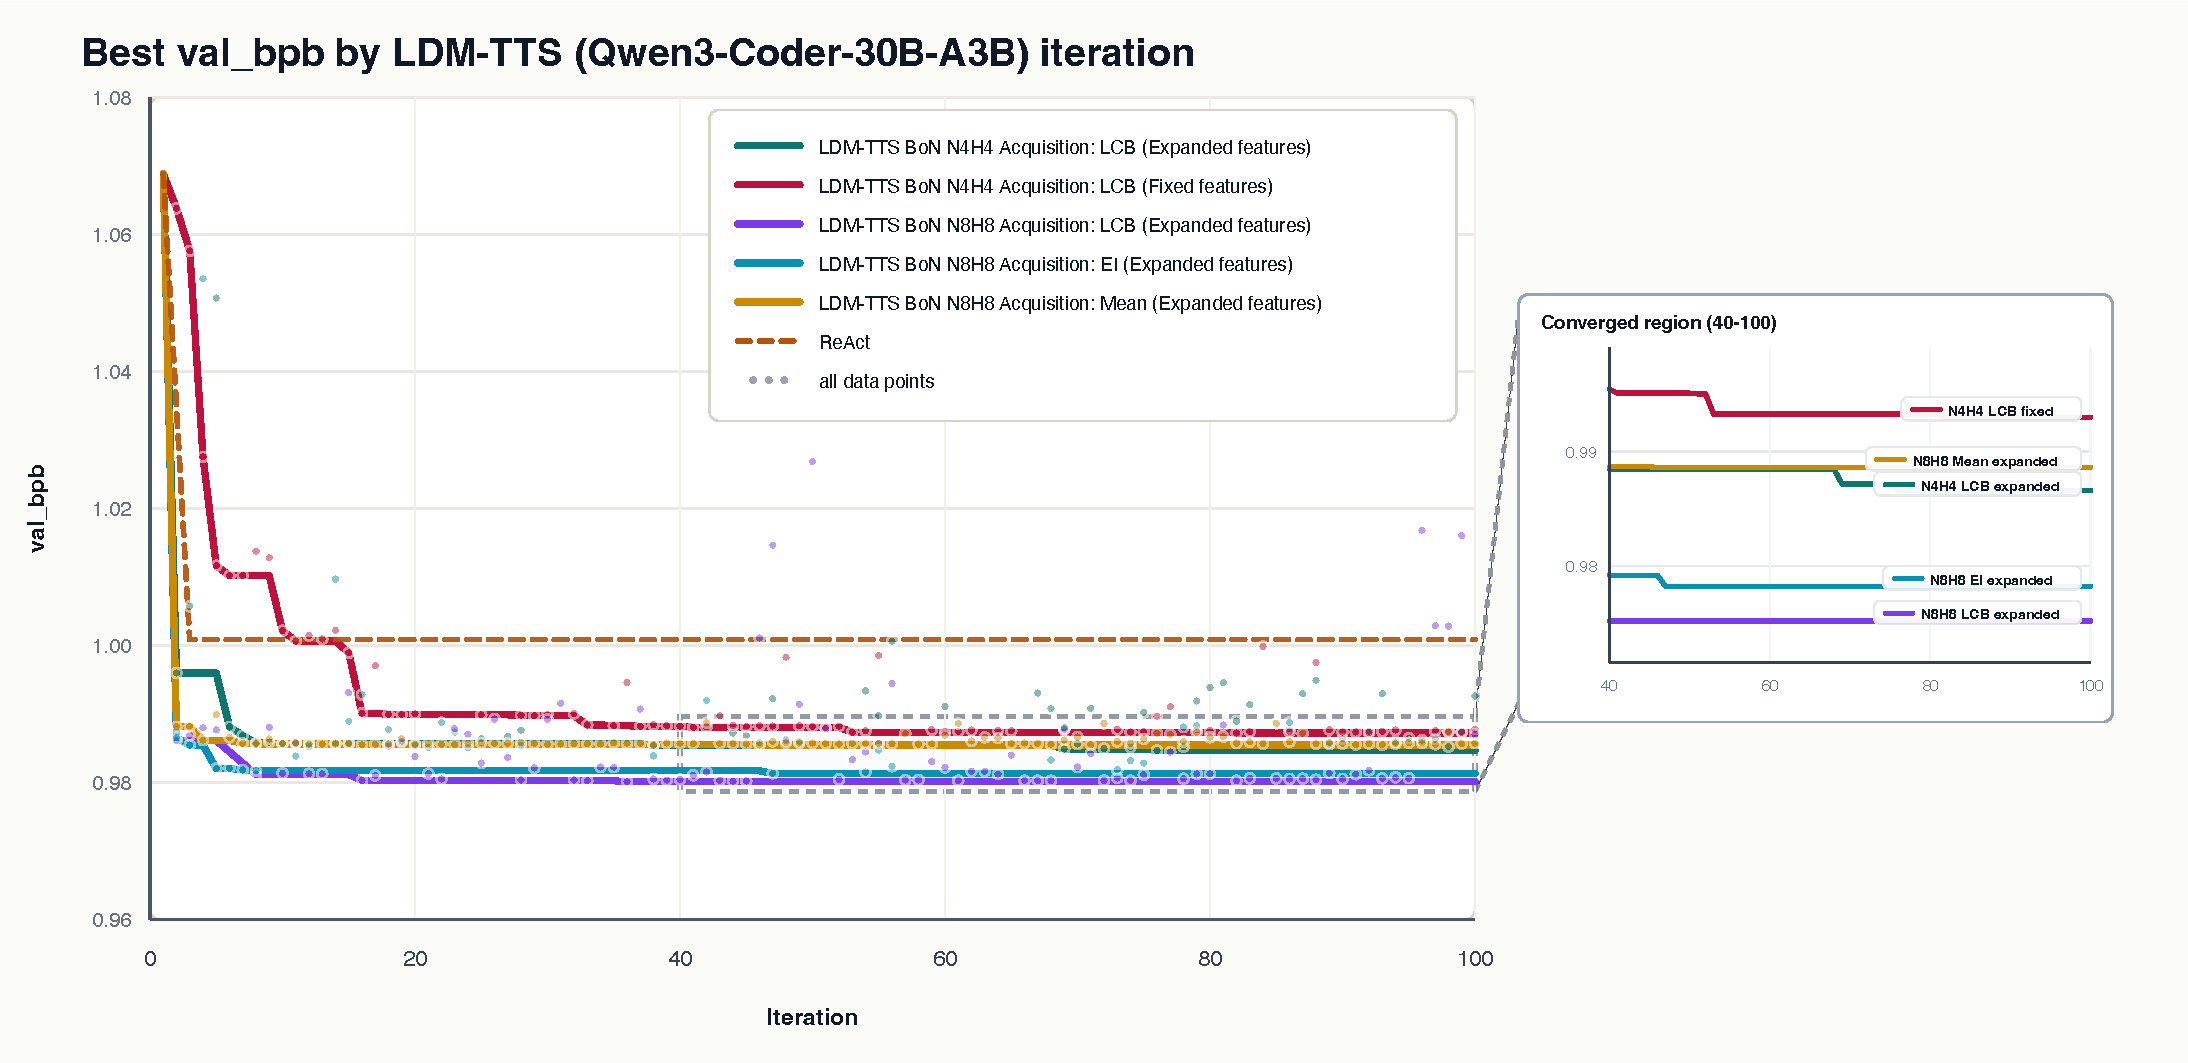
\includegraphics[width=\linewidth]{figure/val_bpb_multi_trial_best_by_iteration.pdf}
    \caption{\textbf{Test-time search ablation on \texttt{autoresearch}.} Best validation \texttt{val\_bpb} found up to iteration $t$ (lower is better). Solid curves are LDM-TTS variants; the dashed curve is a ReAct-style no-acquisition reference \citep{yao2022react}; gray points are all evaluated candidate programs. Each LDM-TTS variant is named \textsc{N$m$H$n$} for its inner budget, where $N$ is the number of candidate programs the LLM proposes and $H$ is the number of hypothesis/refinement branches each candidate is expanded into. }
    \label{fig:abl-autoresearch}
\end{figure}

Figure~\ref{fig:abl-autoresearch} gives three conclusions. First, \emph{increasing the test-time search budget helps}. The \textsc{N8H8} expanded-feature curve reaches the best plateau, while the lower-budget \textsc{N4H4} variants converge higher. Since the outer training budget is unchanged, this improvement comes from spending more cheap computation before each expensive evaluation. Second, \emph{dynamic feature expansion helps}, as \texttt{autoresearch} is not a fixed-dimensional hyperparameter problem. When the agent discovers a new mechanism, such as sparse memory or a new schedule family, the surrogate needs new coordinates on which to model it; fixed features compress those mechanisms into residual noise and produce weaker acquisition guidance. Third, \emph{the acquisition itself matters}. Posterior-mean search is competitive early because it exploits the most promising known direction, but it plateaus above EI and the uncertainty-aware acquisition. EI improves on mean-only selection by rewarding improvement over the incumbent, while the uncertainty-aware value performs best because it deliberately allocates part of the test-time budget to under-modelled program families. These results validate the central claim that the LLM is the semantic search engine, yet the calibrated acquisition is the value that makes additional test-time compute useful.

The same suite of test-time budget ablation sweeps was also conducted for the scientific design tasks detailed in \S\ref{sec:cs-molecule-results} and \S\ref{sec:cs-antibody-results}, with full results presented in Appendix~\ref{app:abl-molecule} and \ref{app:abl-antibody}, respectively. For molecular design, a clear trend emerges: larger search budgets yield more effective discovery. This pattern is weaker for antibody design, where the scaling effect is small in magnitude even though the optimum remains target-dependent across antigens; see Appendix~\ref{app:abl-antibody} for the per-target curves. The root cause is that the underlying large language model lacks specialised domain expertise, rendering its candidate proposals near-random. We further perform comparisons across different acquisition functions. Our results demonstrate that, given a sufficiently large search budget, well-chosen acquisition functions deliver consistent performance gains for both molecular and antibody design. Notably, the mean acquisition (a $0.5/0.5$ scalarisation of the Vina and activity objectives) outperforms EHVI under low search budgets for molecular design. The mechanism is bandwidth: EHVI is built on the strict Pareto frontier and therefore needs a large screening budget to be effective, while mean-style acquisitions collapse the two objectives into one scalar and at small budgets the per-step randomness from a thin screening budget partially substitutes for the missing Pareto signal.

\subsubsection{Hyperparameter sensitivity}

We next study the sensitivity of LDM to its two temperature parameters on the KRAS G12D molecular design task of \S\ref{sec:cs-molecule-results}. Here, the decoding parameter $\alpha$, which is the LLM sampling temperature $T_{\mathrm{LLM}}$, controls the diversity of LLM-generated SMILES candidates, while the acquisition temperature $\eta$ controls the strength of acquisition-guided selection. As $\eta\to0$ the policy collapses to the raw LLM reservoir and as $\eta\to\infty$ it reduces to acquisition-function argmax ($\eta=\infty$ in the experiments below).

\begin{figure*}[htbp]
    \centering
    \begin{subfigure}[t]{0.48\textwidth}
        \centering
        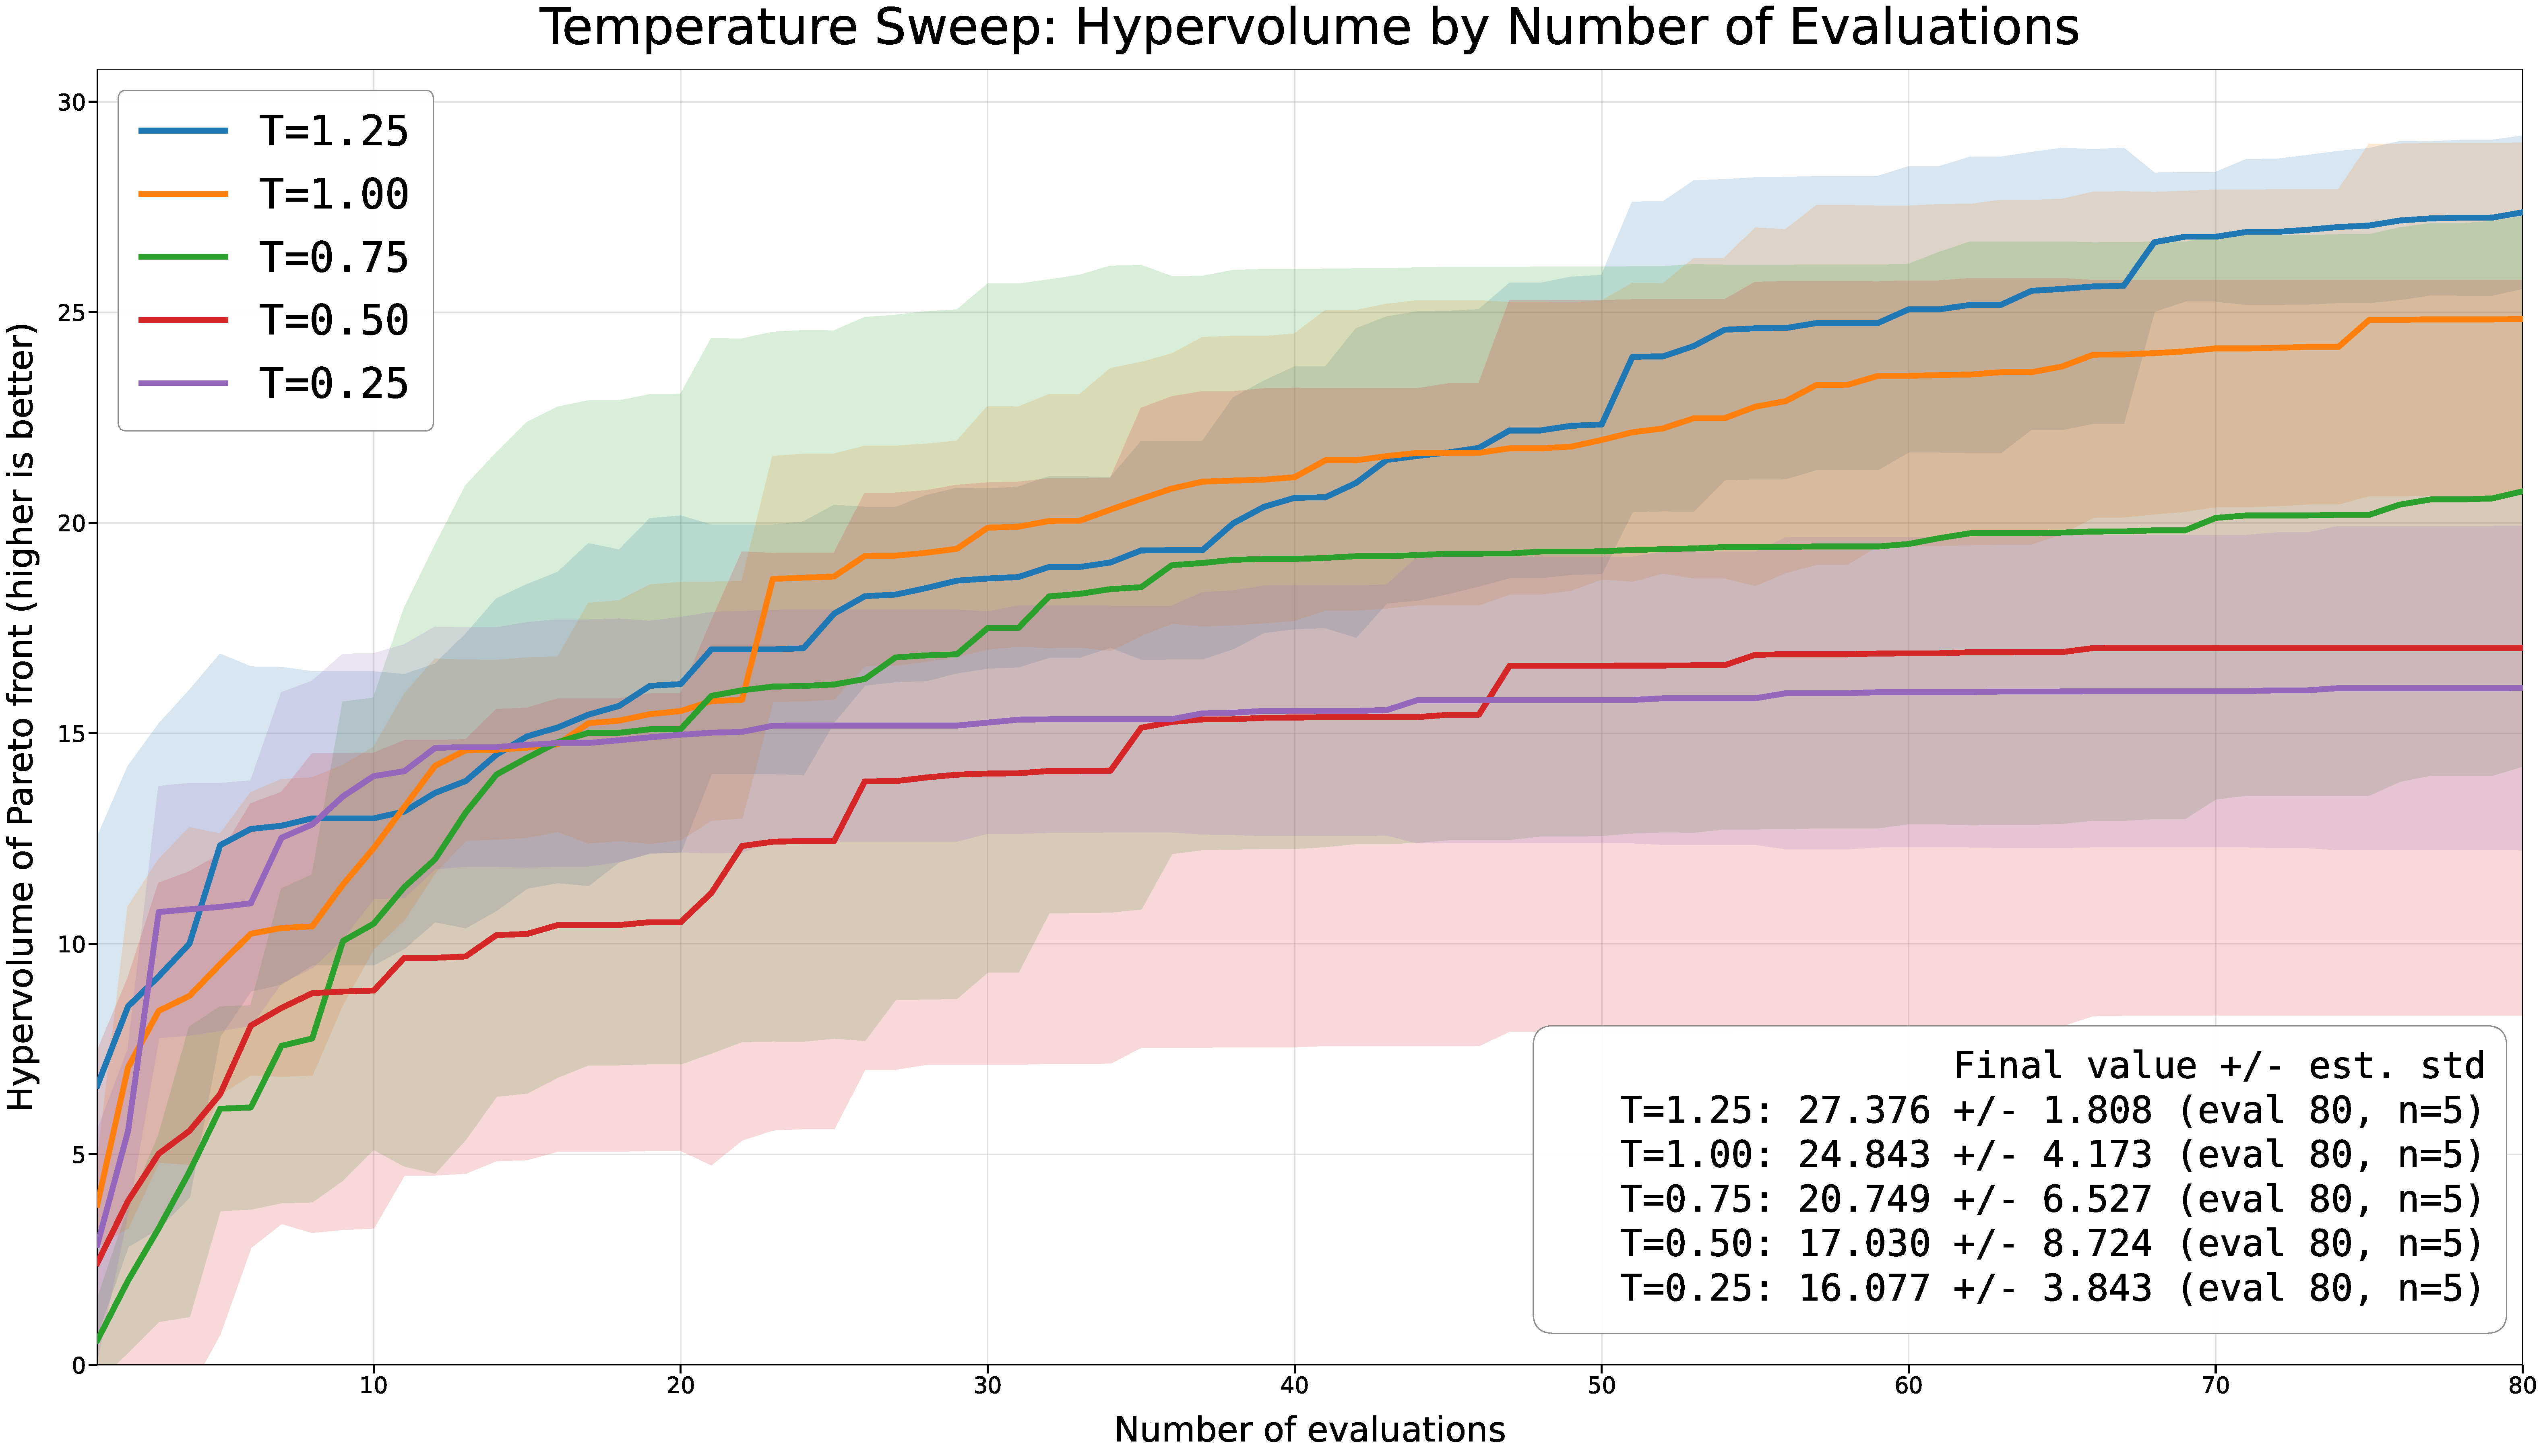
\includegraphics[width=\linewidth]{figure/ldm_molecule_temperature_sweep.pdf}
        \caption{Effect of LLM sampling temperature $T_{\mathrm{LLM}}$ with fixed acquisition temperature $\eta=1$.}
        \label{fig:molecule-temperature-ablation}
    \end{subfigure}
    \hfill
    \begin{subfigure}[t]{0.48\textwidth}
        \centering
        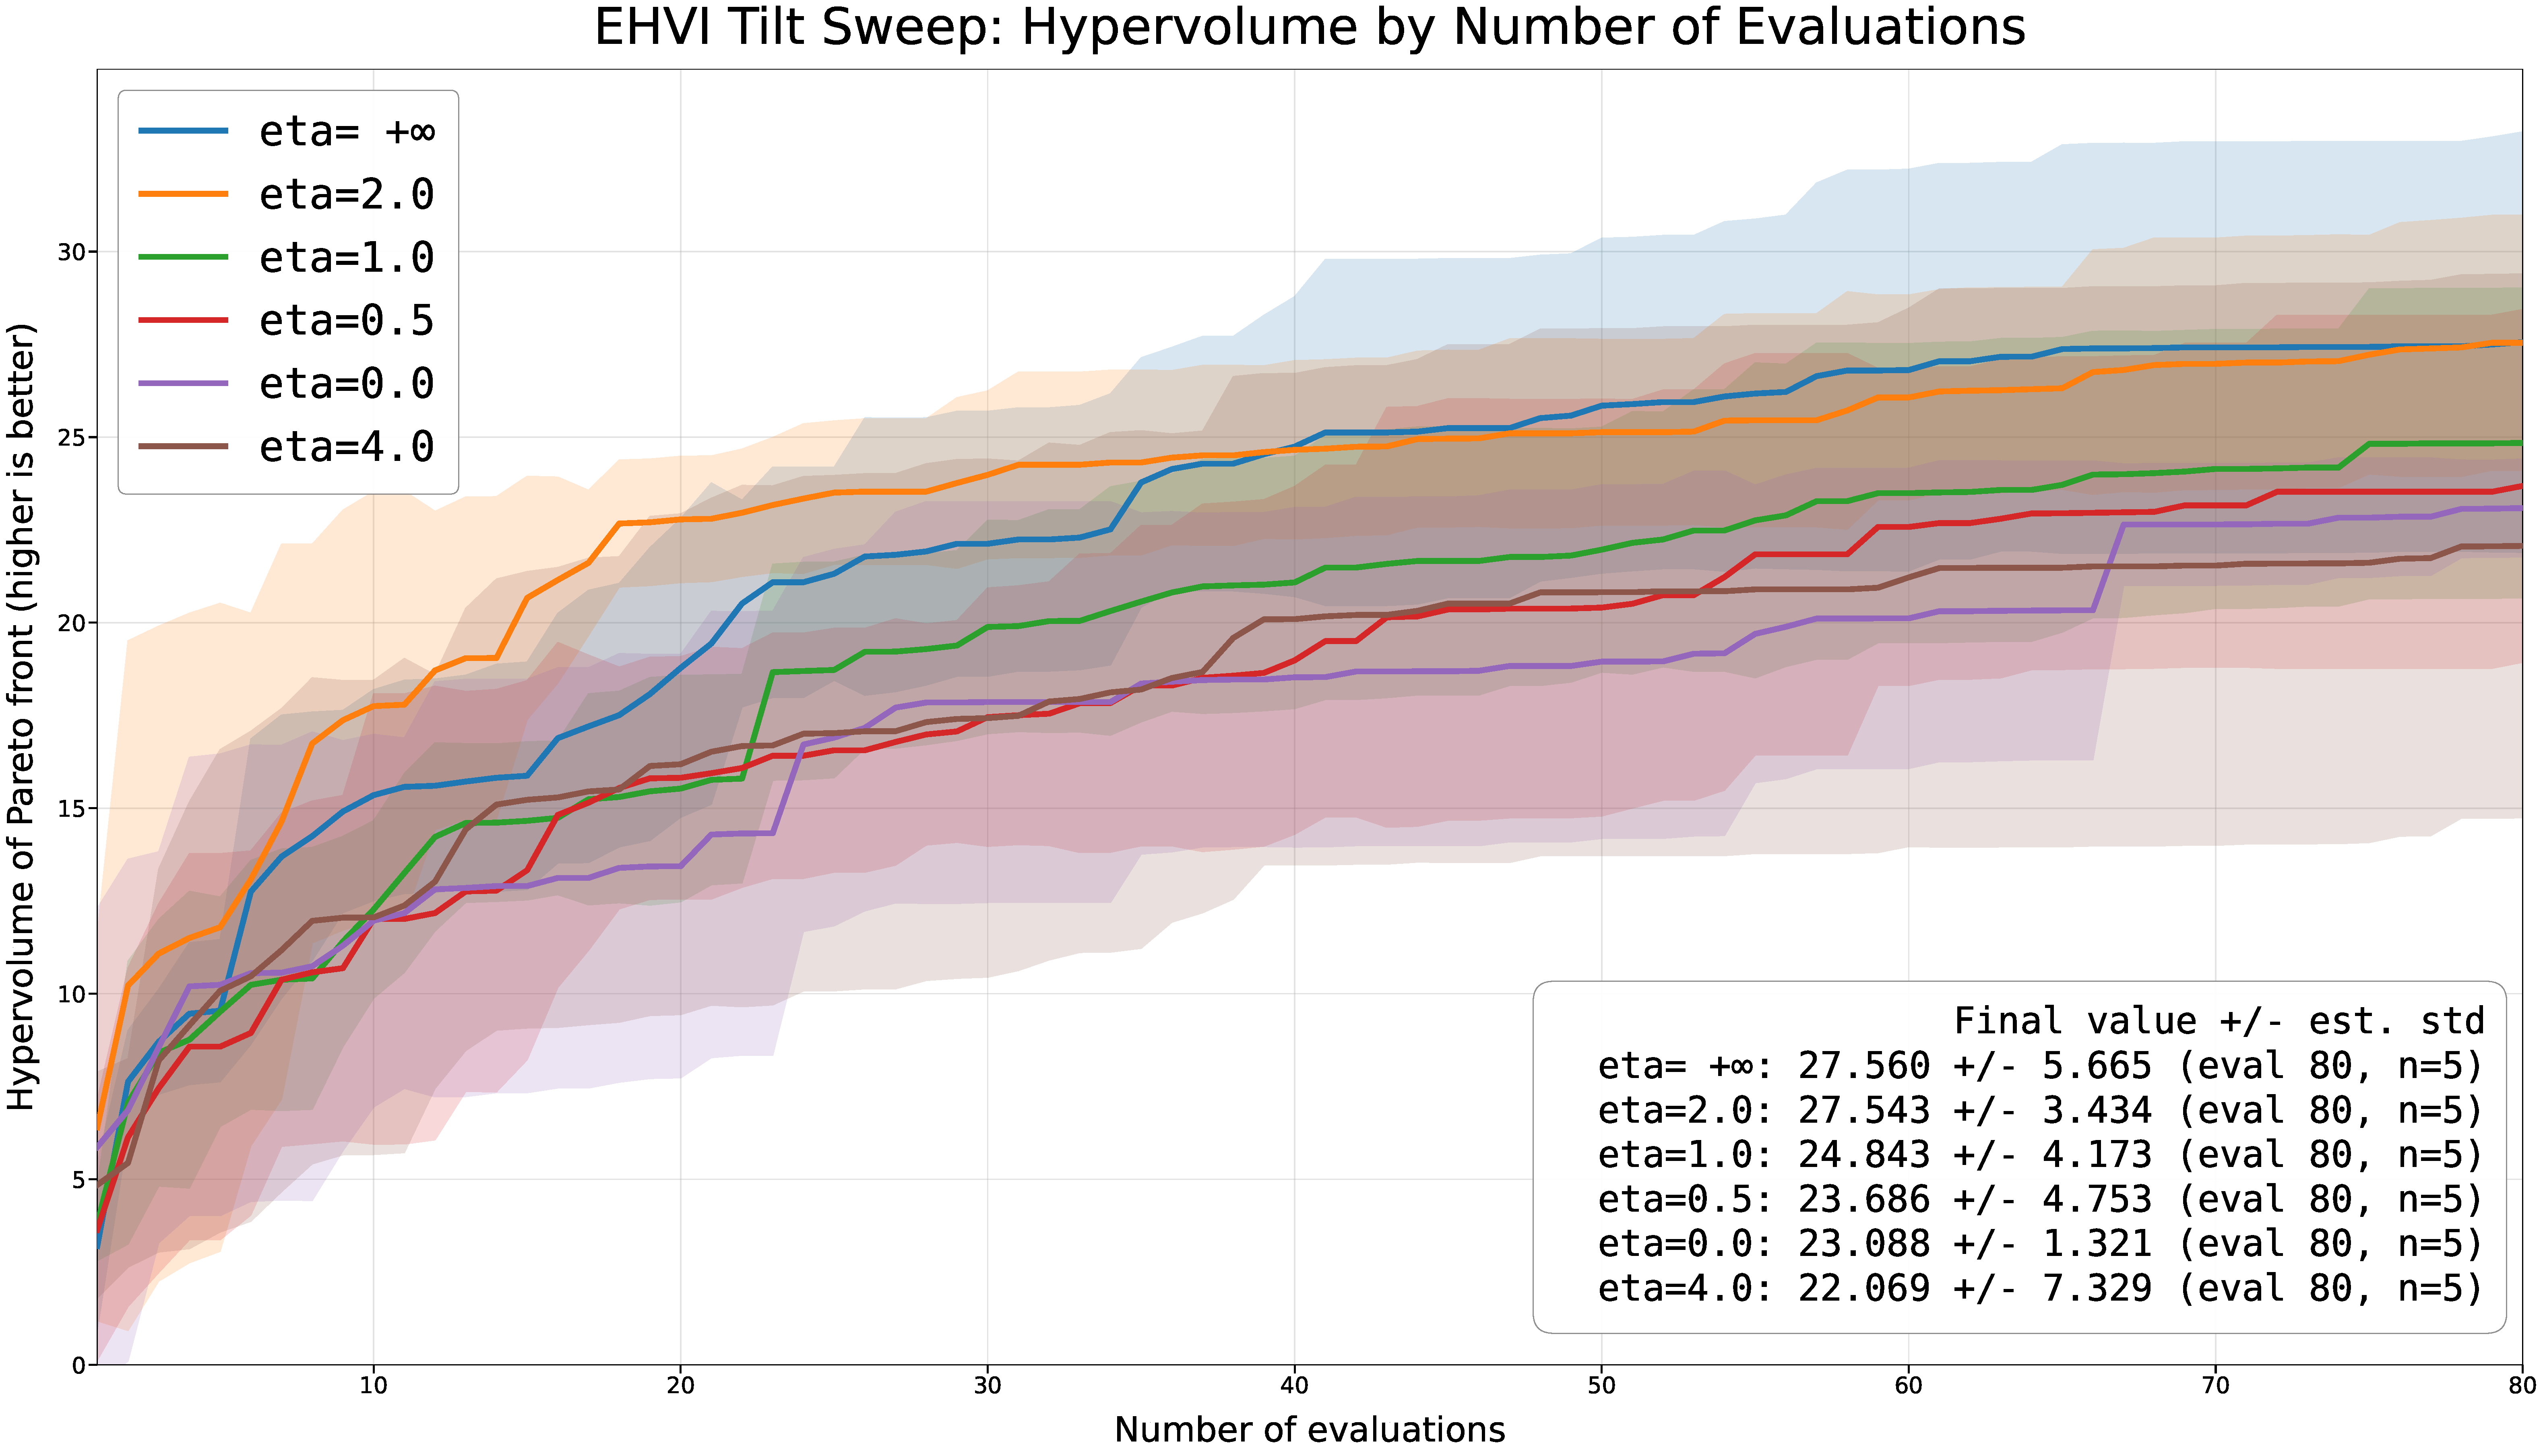
\includegraphics[width=\linewidth]{figure/ldm_molecule_eta_sweep.pdf}
        \caption{Effect of acquisition temperature $\eta$ with fixed LLM sampling temperature $T_{\mathrm{LLM}}=1$.}
        \label{fig:molecule-eta-ablation}
    \end{subfigure}

    \caption{\textbf{Hyperparameter ablations of LDM-TTS on molecular design.} Each curve reports the hypervolume of the Pareto front over the evaluation trajectory. Higher values indicate better multi-objective optimization performance.}
    \label{fig:molecule-temperature-eta-ablation}
\end{figure*}

For the LLM sampling temperature ablation, we fix $\eta=1$ and vary the LLM-decoding temperature $T_{\mathrm{LLM}}$ in $\{0.25, 0.5, 0.75, 1, 1.25\}$. As shown in Figure~\ref{fig:molecule-temperature-ablation}, increasing $T_{\mathrm{LLM}}$ generally improves the final optimization performance: the setting $T_{\mathrm{LLM}}=1.25$ achieves the highest final hypervolume, while lower temperatures degrade performance. For the acquisition temperature ablation, we fix $T_{\mathrm{LLM}}=1$ and vary $\eta\in\{0,0.5,1,\infty\}$. Figure~\ref{fig:molecule-eta-ablation} shows that increasing $\eta$ generally improves the final hypervolume. Overall, on molecular design both sufficient LLM exploration and effective acquisition guidance are necessary for LDM, with the acquisition tilt $\eta$ acting as the dominant driver of final Pareto-front expansion.

Antibody CDRH3 design (\S\ref{sec:cs-antibody-results}) yields distinct overall behaviour. The open-source LLM lacks biological sequence domain priors, generating nearly random candidate sequences across the vast search space. While policy-based LDM variants incorporate implicit acquisition-guided sampling to expand promising candidate regions, this diminishes the standalone impact of test-time acquisition reweighting. Therefore, global hyperparameter sweeps over sampling and acquisition temperatures reveal negligible performance sensitivity. This aligns with the core finding from \S\ref{sec:cs-antibody-results}: policy-mode LDM outperforms direct generation chiefly via built-in structural LLM priors instead of acquisition weighting. Full temperature ablation plots for antibody design are provided in Appendix~\ref{app:abl-hyper-ldm}.

% ============================================================
\subsection{Overall Discussion}
\label{sec:overall-discussion}

Collectively, the three case studies validate LDM as a general approach for model-based scientific discovery across distinct structured search domains, with consistent core conclusions emerging from all experimental setups.

First, combining calibrated Bayesian surrogate acquisition with LLM-driven inference-time search consistently outperforms standalone LLMs and vanilla Bayesian optimisation. LLMs supply native semantic generation over complex discrete spaces where BO cannot easily propose valid candidates, while Gaussian process surrogates deliver reliable uncertainty-aware value signals missing from uncalibrated LLM self-scoring. Neither component alone reproduces the full performance gains observed in the integrated LDM pipeline.

Second, the optimal LLM operating mode is domain-dependent, governed by the strength of the model’s pre-trained domain priors and the structure of the design space. For sparsely covered sequence spaces such as antibody CDRH3, policy-mode LLM search expands exploration coverage by defining local search zones. For domains with rich LLM pre-training data (code, SMILES), large-batch direct generation achieves superior Pareto/affinity improvements. The unified tilted distribution formulation accommodates both paradigms without modification to the underlying acquisition-guided optimisation logic.

Third, the three-way exploit–explore–discover trichotomy differentiates LDM from classic BO methods limited to two-way trade-offs. In all benchmarks, baseline systems lacking a generative reservoir eventually stagnate at fixed performance ceilings. LDM’s discovery mechanism breaks these plateaus by extending the set of candidate designs under evaluation whenever local optimisation yields no further gains, lifting the upper bound of achievable objective values over repeated iterations.

Fourth, the ablation and fine-tuning studies in \S\ref{sec:ablation-main} and \S\ref{sec:finetune-experiments} clarify why the framework works. Test-time search helps only when the additional inference-time compute is filtered by a calibrated, uncertainty-aware acquisition rather than by language plausibility, and the surrogate must track the search space as it evolves. When the LLM reservoir is itself weakly informative, as in antibody CDRH3 design, acquisition reweighting adds little beyond the policy's structural search. The fine-tuning results further show that the tilted search policy can be distilled into a single lightweight proposer, and that grounding distilled actions in surrogate value improves both same-domain and cross-task transfer. Together, these findings indicate that LDM's gains reflect a learnable discovery strategy rather than task-specific memorisation.

Finally, the empirical evidence reinforces this paper’s central framing: scientific design is an inverse decision problem rather than a forward prediction task. LDM constructs a learned surrogate landscape and searches within it for target-compliant structures, rather than only predicting properties from given inputs. The LLM acts as a flexible inference-time optimiser for Bayesian acquisition functions over semantically structured discrete spaces, not a replacement for principled uncertainty-aware optimisation. Remaining limitations include the cubic computational cost of exact Gaussian Processes at large evaluation budgets, and potential surrogate reward hacking. Even with these constraints, consistent performance improvements across program search, protein design and medicinal chemistry confirm that acquisition-guided LLM inference provides a broadly applicable foundation for autonomous closed-loop scientific discovery.